\documentclass{article}
\PassOptionsToPackage{numbers}{natbib}
\usepackage[preprint]{neurips_2026}
\usepackage[utf8]{inputenc}
\usepackage[T1]{fontenc}
\usepackage{microtype}
\usepackage{amsmath,amssymb,amsfonts,amsthm,mathtools,bm,mathrsfs}
\usepackage{booktabs,array,multirow}
\usepackage{xcolor,graphicx,hyperref}
\usepackage{enumitem}
\usepackage{tikz}
\usetikzlibrary{arrows.meta,positioning,calc}
\hypersetup{colorlinks=true,linkcolor=blue!55!black,citecolor=blue!55!black,urlcolor=blue!55!black}

\definecolor{widthblue}{HTML}{276FBF}
\definecolor{rankred}{HTML}{D1495B}
\definecolor{transportgray}{HTML}{565D67}

\newtheorem{theorem}{Theorem}[section]
\newtheorem{proposition}[theorem]{Proposition}
\newtheorem{lemma}[theorem]{Lemma}
\newtheorem{corollary}[theorem]{Corollary}
\newtheorem{definition}[theorem]{Definition}
\newtheorem{assumption}[theorem]{Assumption}
\newtheorem{remark}[theorem]{Remark}

\newcommand{\E}{\mathbb E}
\newcommand{\R}{\mathbb R}
\newcommand{\cP}{\mathcal P}
\newcommand{\cS}{\mathcal S}
\newcommand{\cA}{\mathcal A}
\newcommand{\Cov}{\operatorname{Cov}}
\newcommand{\Var}{\operatorname{Var}}
\newcommand{\cum}{\operatorname{cum}}
\newcommand{\Tr}{\operatorname{Tr}}
\newcommand{\diag}{\operatorname{diag}}
\newcommand{\rank}{\operatorname{rank}}
\newcommand{\relu}{\operatorname{ReLU}}
\newcommand{\one}{\mathbf 1}
\newcommand{\dd}{\,\mathrm d}
\newcommand{\ind}{\mathbf 1}
\newcommand{\NTK}{\mathrm{NTK}}
\newcommand{\NNGP}{\mathrm{NNGP}}
\newcommand{\GOE}{\mathrm{GOE}}
\newcommand{\op}{\mathrm{op}}

\title{Exact Depth Scaling and Low-Rank Feynman Calculus\\
for Multi-Component Multilayer Networks}
\author{Anonymous Authors}

\begin{document}
\maketitle

\begin{abstract}
The depth exponents displayed in recent finite-width neural-tangent-kernel
(NTK) Feynman plots were obtained by Monte Carlo regression, and their
noninteger values were not exact critical powers.  We close this gap for
fully connected critical ReLU networks and extend the diagrammatics to
multi-component and multilayer neural networks (MMNNs), whose blocks have the
form
\(h_\ell=A_\ell\relu(W_\ell h_{\ell-1})\), with frozen \(W_\ell\) and
trainable \(A_\ell\).

First, we derive a pathwise matrix-valued NTK recursion for the actual MMNN,
without a Gaussian-process or infinite-rank approximation.  Concatenating
two blocks inserts the rank-\(r\) tangent metric
\(G=XX^\top/r\).  Its moments and connected cumulants are computed at every
valence by a closed Wick-pairing formula.  A QR decomposition separates this
vertex into an independent Wishart radial part and a Haar--Stiefel
orientation; orthogonal Weingarten calculus gives an exact all-valence
formula for the latter.  This distinction corrects the common projector-only
replacement, which is exact only after whitening the induced parameter
metric.

Second, working directly with the connected-cumulant definitions of
Guillen--Misof--Gerken, we solve the deterministic leading-width ReLU
recursions for the five non-MMNN four-index tensors \(V,D,F,A,B\).  For every fixed non-collinear input set,
all components plotted in Guillen--Misof--Gerken have the attained powers
\[
V=\Theta(L),\qquad D,F=\Theta(L^2),\qquad A,B=\Theta(L^3).
\]
We give every leading coefficient in closed form, prove non-cancellation,
and derive the logarithmic critical drift
\(\theta_{ab,L}=3\pi/[L+(3/2)\log L+C_{ab}+o(1)]\).
Applying the original regression windows to our exact recursion explains the
reported effective slopes between \(1.19\) and \(3.78\) without introducing
new anomalous powers.

Third, we lift these five cumulants to the MMNN component indices.  Their
diagrams split into a width-colored sector and a bottleneck-rank-colored
sector.  In the controlled double expansion, their attained depth powers are
again \(1,2,2,3,3\), while their amplitudes scale as \(1/n+1/r\) for Gaussian
MMNNs and as \(1/n+\gamma_{n,r}\) for the whitened Stiefel model.  We give the
exact contraction formula for each rank coefficient and delimit the
perturbative depth window.

Fourth, we show that the complete MMNN tangent feature is an exact
concatenation of low-rank Kronecker-Gram blocks.  Under the
Benigni--Paquette quadratic-scaling hypotheses, its spectrum is one
Marchenko--Pastur map of the full block population covariance.  For
homogeneous decoupled blocks we obtain the closed law
\(\mu_{\rm MP}^{\gamma_1/L}\boxtimes(L\cdot)_\#\mu_{\nu,\varphi}\) and its
exact linear spectral response.

Fifth, we connect the diagrammatics to the symmetry-derived neural quadratic
form (NQF) of Liu Ziyin, Xu, Poggio, and Chuang.  We identify its structure
matrix with a two-leg Landau vertex and \(\mathsf M=WW^\top\) with a dynamic
Gram order parameter.  All chains of quadratic vertices close exactly on
\(\mathsf M\); in the commuting orthogonal-feature sector this gives the
complete finite-sample NTK spectrum and logistic mode ignition.  Combining
the exact Wishart and Haar--Stiefel seed laws with this flow yields explicit
finite-rank ignition-time distributions, including exact cancellation of
clock disorder at the full-rank Stiefel endpoint.  We state precisely why
this is an exact resummation for the NQF but only a local normal form for a
nonlinear MMNN.

Finally, the finite-size tensor covariance is resummed spectrally.  In an isotropic
large-rank sector, its connected-cumulant hierarchy yields a deformed-Wigner
Dyson equation.  We compute limiting trace moments, eigenvalue density, and
basis-resolved eigenvector overlaps, and insert the resulting local spectral
measures into power-law random-feature learning dynamics.  A
positive-semidefinite deformation shows that finite-rank mixing need not
always move early stopping earlier: the direction is determined by the full
diagrammatic covariance.  All symbolic identities, deterministic recursions,
spectral solvers, and figures are accompanied by executable tests.
\end{abstract}

\section{Introduction}

Finite-width neural networks are perturbations of their infinite-width
kernels, but the perturbation is structured.  Its entries share neurons,
gates, backpropagated paths, and---in a low-rank network---the same random
subspaces.  Entrywise central-limit intuition is therefore insufficient for
depth scaling or spectral questions.  Feynman diagrams provide the right
bookkeeping: channel loops determine powers of width or rank, while connected
vertices determine which tensor cumulants survive.

Dyer and Gur-Ari established the large-width diagrammatic power counting and
related derivative-tensor contractions to spectral moments
\citep{DyerGurAri2019}.  Those relations do not imply a universal Wigner law
for nonlinear NTKs: the covariance sector must first be computed.  Our
spectral analysis therefore uses their moment viewpoint but closes it with a
covariance-specific matrix Dyson equation.

Two recent developments make a sharper theory possible.  Guillen, Misof, and
Gerken derive exact recursive expressions for the leading finite-width
tensors of deep nonlinear networks and report componentwise depth slopes from
finite-network Monte Carlo experiments \citep{FeynmanNTK2026}.  Separately,
MMNNs compose shallow random-feature maps
\(A_\ell\sigma(W_\ell\cdot+b_\ell)+c_\ell\), training the component matrices
\(A_\ell,c_\ell\) while freezing \(W_\ell,b_\ell\) \citep{MMNN2024}.  The
adjacent product \(W_{\ell+1}A_\ell\) is a low-rank effective weight with a
frozen left and trainable right factor.  The natural question is whether the
dense Feynman tensor theory can be made exact in depth and extended to this
alternating width--rank architecture.

Benigni and Paquette compute an asymptotic eigenvalue distribution for a
two-layer NTK in the quadratic sample--parameter scaling
\citep{BenigniPaquette2025}.  That result is complementary spectral input; it
does not by itself supply a multilayer concatenation identity.  Here the
concatenation rule instead follows pathwise from the chain rule.

The first answer is a correction: the slopes printed in the depth plots are
not exact exponents.  They are least-squares slopes of empirical finite-width
tensors over depths at most \(30\).  At critical ReLU initialization, distinct
inputs approach perfect correlation only as \(L^{-2}\), with a logarithmic
drift.  Consequently a tensor with true leading behavior \(cL^p\) can have a
substantial effective slope different from \(p\) over this window.  We
evaluate the exact deterministic recursions and prove that the five powers
are the integers \(1,2,2,3,3\), component by component.

The second answer is architectural.  A Gaussian frozen factor is not a Haar
projector.  Writing \(X=QR\) gives
\[
\frac1rXX^\top=Q\frac{RR^\top}{r}Q^\top.
\]
The orientation \(Q\) is Haar--Stiefel and the radial matrix \(RR^\top\) is
Wishart, independently.  Dropping the radial vertex changes finite-rank
moments and the Euclidean tangent metric.  We therefore give parallel exact
rules for (i) the Gaussian Gram vertex of the actual MMNN and (ii) the
whitened Stiefel-projector surrogate.  The former has connected \(k\)-vertex
cumulants of order \(r^{1-k}\); the latter has finite-\((n,r)\) rational
Weingarten weights and an exact identity endpoint at \(r=n\).

The third answer concerns eigenvalues.  Weingarten calculus determines Haar
orientation averages and eigenvector moments, but it does not by itself
diagonalize a nonlinear NTK.  The tensor recursion first supplies the
covariance operator of the NTK correction.  A matrix Dyson equation then
resums the leading spectral diagrams.  In the isotropic case this reduces to
the Pastur equation for a deformed Wigner matrix; in the general correlated
case it is an operator-valued Dyson equation.  This yields eigenvalue density
and eigenvector overlaps from the same tensor data.

In the quadratic sample--parameter regime there is a second, nonperturbative
base law.  The Benigni--Paquette theorem applies to one Kronecker tangent
block.  The exact pathwise concatenation shows that a deep MMNN is the Gram
matrix of all such transported blocks at once.  A single MP map therefore
acts on their full block population covariance; the off-diagonal layer
blocks determine whether the simpler homogeneous formula is valid.

A third simplification occurs near a symmetry-fixed parameter origin.
Liu Ziyin, Xu, Poggio, and Chuang prove that permutation symmetry together
with their zero-gradient-at-zero condition forces the leading nonconstant
term to be a quadratic form \(\Tr(WW^\top\mathscr A_x)\)
\citep{NQF2026}.  This is a Landau normal form, not a claim that an arbitrary
network is globally quadratic.  In diagrammatic language \(\mathscr A_x\)
is a deterministic two-leg vertex.  Because its gradient is linear in
\(W\), every repeated insertion closes on the dynamic Gram matrix
\(\mathsf M=WW^\top\).  This produces exact training-time resummations inside
the NQF and a controlled local sector to be matched to the finite-width and
finite-rank initialization diagrams developed here.

\paragraph{Main results.}
\begin{enumerate}[leftmargin=1.55em]
\item We prove the exact pathwise MMNN NTK recursion, Theorem
\ref{thm:pathwise-mmnn}, and identify the concatenated low-rank tangent
metric without changing the architecture.
\item We derive all-valence Gaussian Gram moment/cumulant rules, Theorem
\ref{thm:gram-wick}, and all-valence Haar-projector Weingarten rules,
Theorem \ref{thm:projector-weingarten}.
\item We give deterministic exact finite-depth ReLU recursions for
\(V,D,F,A,B\), including closed ReLU transport Hessians and a deterministic
Tallis--Plackett evaluation of every source moment.
\item We prove attained componentwise powers and closed leading
coefficients, Theorem \ref{thm:componentwise-powers}.  In particular none of
the thirty plotted components cancels at leading order.
\item We compute the same finite-window regressions used in the original
plots and separate them from the exact asymptotic powers.
\item We define the MMNN analogues of the same five connected cumulants and
prove their two-color depth hierarchy, Theorem \ref{thm:mmnn-powers}.
\item We prove the exact tangent-feature concatenation and, under the stated
quadratic-scaling concentration hypotheses, derive the multilayer
Benigni--Paquette law and its spectral response, Theorem
\ref{thm:mmnn-bp-law} and Corollary
\ref{cor:bp-homogeneous-concatenation}.
\item We give an NQF--MMNN dictionary, prove the exact quadratic-vertex
resummation and dynamic NTK formula, and compute the full spectrum and
finite-rank mode-ignition clocks in the orthogonal-feature sector, Theorems
\ref{thm:nqf-resummation}, \ref{thm:nqf-spectrum}, and
\ref{thm:nqf-clock-disorder}.
\item We derive spectral moments, the Dyson resolvent, eigenvalue density,
and local eigenvector overlaps, and apply them to power-law scaling and early
stopping.
\end{enumerate}

\paragraph{Scope.}
The closed rational coefficients in Theorem
\ref{thm:componentwise-powers} concern the leading \(1/n\) coefficient of
the dense critical ReLU expansion.  The MMNN Feynman rules are exact at
finite width and rank, while its exponent theorem is a controlled joint
\(1/n,1/r\) expansion; a fixed-rank, arbitrarily deep limit is outside that
expansion.  The quadratic-scaling law additionally requires convergence and
quadratic-form concentration of the transported population covariance; its
direct application to the discontinuous ReLU derivative requires a
universality extension.  The Wigner reduction in Section \ref{sec:spectral}
requires a separate large-data isotropy assumption.  We distinguish exact
identities, asymptotic theorems, and conditional random-matrix reductions
throughout.  Nonnegative matrix factorization constraints are not present in
the MMNN architecture studied in \citep{MMNN2024}; adding positivity would
replace the tangent space by an active cone and requires a separate theory.
The NQF statements add a second, independent scope condition: closure is
exact for the quadratic model, whereas transferring it to the original
nonlinear network is local in parameter norm.  Moreover, a single MMNN block
trained only through its right factor lies in the linear part of the general
normal form; a pure \(\mathsf M\)-sector first appears for a bilinear pair of
trainable blocks or for a layerwise deep NQF.

\section{The actual MMNN and its pathwise NTK}
\label{sec:mmnn}

Let \(r_0\) be the input dimension, \(r_L\) the output dimension, and
\(n_\ell\) the random-feature width of block \(\ell\).  We use the normalized
bias-free model
\begin{align}
z_\ell(x)&=\frac{1}{\sqrt{r_{\ell-1}}}W_\ell h_{\ell-1}(x),
&W_\ell&\in\R^{n_\ell\times r_{\ell-1}},\label{eq:mmnn-z}\\
h_\ell(x)&=\frac{1}{\sqrt{n_\ell}}A_\ell\phi(z_\ell(x))+c_\ell,
&A_\ell&\in\R^{r_\ell\times n_\ell}.
\label{eq:mmnn-h}
\end{align}
The frozen variables are \(W_\ell\); the trainable variables are
\(A_\ell,c_\ell\).  Scale constants can be absorbed into \(W,A\) and are
restored when needed.  Define
\begin{align}
q_\ell(x,y)&=\frac1{n_\ell}
\phi(z_\ell(x))^\top\phi(z_\ell(y))+1,\label{eq:q-direct}\\
J_\ell(x)&=\frac{1}{\sqrt{n_\ell r_{\ell-1}}}
A_\ell D_\ell(x)W_\ell,
\qquad D_\ell(x)=\diag\phi'(z_\ell(x)).\label{eq:mmnn-J}
\end{align}

\begin{theorem}[Exact pathwise MMNN NTK recursion]
\label{thm:pathwise-mmnn}
For every realization of the weights, every finite width and rank, and all
inputs \(x,y\), the matrix-valued NTK with respect to
\(\{A_s,c_s:s\le\ell\}\) satisfies
\begin{equation}
\Theta_\ell(x,y)=q_\ell(x,y)I_{r_\ell}
+J_\ell(x)\Theta_{\ell-1}(x,y)J_\ell(y)^\top,
\qquad \Theta_0=0.
\label{eq:pathwise-ntk}
\end{equation}
No independence, Gaussian-process, or infinite-width limit is used.
\end{theorem}

Equation \eqref{eq:pathwise-ntk} is the base object for MMNN diagrams.  A
direct vertex is born when \(A_\ell,c_\ell\) are differentiated; earlier
vertices are transported by the random Jacobian \(J_\ell\).  It also makes
the low-rank metric precise.  Combining adjacent blocks produces the
effective matrix
\begin{equation}
M_{\ell+1}=\frac1{\sqrt{r_\ell}}W_{\ell+1}A_\ell.
\end{equation}
For fixed right indices \(u,v\), contraction of two derivatives with respect
to \(A_\ell\) gives
\begin{equation}
\sum_{a,k}
\frac{\partial M_{iu}}{\partial (A_\ell)_{ak}}
\frac{\partial M_{jv}}{\partial (A_\ell)_{ak}}
=\delta_{uv}G_{ij},
\qquad G=\frac1{r_\ell}W_{\ell+1}W_{\ell+1}^\top.
\label{eq:gram-tangent-metric}
\end{equation}
Thus the correct low-rank line is a Gram matrix.  If
\(W=X\) has iid standard Gaussian entries, it is normalized Wishart.  If
\(W=\sqrt n\,U\) with \(U^\top U=I_r\), it is the normalized projector
\(G=(n/r)UU^\top\).  These ensembles agree in mean but not in higher moments.

\begin{figure}[t]
\centering
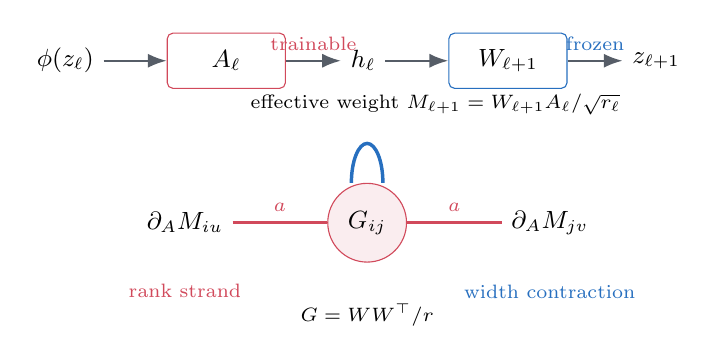
\begin{tikzpicture}[
  >=Latex,
  box/.style={draw,rounded corners=2pt,minimum height=7mm,minimum width=15mm,
    fill=white,font=\small},
  flow/.style={->,line width=0.85pt,color=transportgray},
  rankline/.style={line width=1.25pt,color=rankred},
  widthline/.style={line width=1.25pt,color=widthblue},
  every node/.style={font=\small}
]
\node (phi) {$\phi(z_\ell)$};
\node[box,draw=rankred,right=8mm of phi] (A) {$A_\ell$};
\node[right=7mm of A] (h) {$h_\ell$};
\node[box,draw=widthblue,right=8mm of h] (W) {$W_{\ell+1}$};
\node[right=7mm of W] (z) {$z_{\ell+1}$};
\draw[flow] (phi)--(A);
\draw[flow] (A)--node[above,font=\scriptsize,color=rankred]{trainable}(h);
\draw[flow] (h)--(W);
\draw[flow] (W)--node[above,font=\scriptsize,color=widthblue]{frozen}(z);
\node[below=3mm of $(h)!0.5!(W)$,font=\scriptsize] {effective weight
  $M_{\ell+1}=W_{\ell+1}A_\ell/\sqrt{r_\ell}$};

\coordinate (leftleg) at ($(A.south)+(0,-17mm)$);
\coordinate (rightleg) at ($(W.south)+(0,-17mm)$);
\node[circle,draw=rankred,fill=rankred!10,minimum size=10mm]
  (gram) at ($(leftleg)!0.5!(rightleg)$) {$G_{ij}$};
\node[left=12mm of gram] (di) {$\partial_A M_{iu}$};
\node[right=12mm of gram] (dj) {$\partial_A M_{jv}$};
\draw[rankline] (di)--node[above,font=\scriptsize]{$a$}(gram);
\draw[rankline] (gram)--node[above,font=\scriptsize]{$a$}(dj);
\draw[widthline] ($(gram.north)+(-2mm,0)$)
  arc[start angle=180,end angle=0,x radius=2mm,y radius=5mm];
\node[below=4mm of gram,font=\scriptsize] {$G=WW^\top/r$};
\node[below=4mm of di,font=\scriptsize,color=rankred] {rank strand};
\node[below=4mm of dj,font=\scriptsize,color=widthblue] {width contraction};
\end{tikzpicture}
\caption{Concatenating two MMNN blocks produces a frozen-left/trainable-right
effective weight.  Contracting two trainable-right tangents creates the
normalized Gram vertex \(G\), whose component strand is red and frozen-feature
contraction is blue.  Gaussian Wick or Stiefel Weingarten rules evaluate this
same vertex without changing the network.}
\label{fig:mmnn-gram-vertex}
\end{figure}

\section{Feynman rules: width loops, rank loops, and connected vertices}
\label{sec:rules}

The alternating indices of an MMNN have two colors.  Greek feature indices
\(\mu\in[n]\) produce width loops; Latin component indices \(a\in[r]\)
produce rank loops.  With iid Gaussian frozen factors,
\begin{equation}
\E W_{\mu a}W_{\nu b}=\delta_{\mu\nu}\delta_{ab}.
\end{equation}
Every Wick contraction therefore closes both a width and a rank strand.  A
connected cumulant of \(k\) empirical feature vertices costs
\(n^{1-k}\), while a connected cumulant of \(k\) Gram vertices costs
\(r^{1-k}\).  A connected MMNN diagram \(\Gamma\) consequently carries
\begin{equation}
\operatorname{wt}(\Gamma)
=n^{-\sum_v(k_v^{(n)}-1)}
r^{-\sum_w(k_w^{(r)}-1)}
\times\operatorname{Contr}(\Gamma),
\label{eq:double-power-counting}
\end{equation}
where \(\operatorname{Contr}(\Gamma)\) contains ReLU source and transport
tensors.  Equation \eqref{eq:double-power-counting} is exact before summing
over layer locations.  Depth powers arise from the number and transport of
allowed vertex insertions.

At first connected order, an actual Gaussian MMNN has width and rank sources
of orders \(1/n\) and \(1/r\); mixed diagrams can correlate their
contractions.  In an isotropic sector this gives
the perturbative scale
\begin{equation}
\varepsilon_{n,r}=\frac{c_n}{n}+\frac{c_r}{r},
\label{eq:actual-mmnn-epsilon}
\end{equation}
with contractions \(c_n,c_r\) fixed by the diagram.  It is generally wrong
to replace \eqref{eq:actual-mmnn-epsilon} by a single projector defect.  For
the whitened Stiefel surrogate the orientation covariance instead contains
the exact defect
\begin{equation}
\gamma_{n,r}=\frac{n(n-r)}{r(n-1)(n+2)},
\label{eq:gamma}
\end{equation}
which vanishes at \(r=n\).  The ordinary width contribution remains.

\section{Non-MMNN theory in the exact tensor framework}
\label{sec:relu-recursion}

This section contains no MMNN or low-rank assumption.  It uses exactly the
neural-index decomposition of Guillen--Misof--Gerken
\citep{FeynmanNTK2026}.  If
\(\Delta\widehat\Theta=\widehat\Theta-\E\widehat\Theta\), their five tensors
are defined by
\begin{align}
\cum(z_{i_1;1},z_{i_2;2},z_{i_3;3},z_{i_4;4})
={}&\frac1{n_{\ell-1}}\big[
\delta_{i_1i_2}\delta_{i_3i_4}V_{1234}
+\delta_{i_1i_3}\delta_{i_2i_4}V_{1324}
+\delta_{i_1i_4}\delta_{i_2i_3}V_{1423}\big],
\label{eq:original-V-definition}\\
\cum(z_{i_1;1},z_{i_2;2},\Delta\widehat\Theta_{i_3i_4;34})
={}&\frac1{n_{\ell-1}}\big[
\delta_{i_1i_2}\delta_{i_3i_4}D_{1234}
+\delta_{i_1i_3}\delta_{i_2i_4}F_{1324}
+\delta_{i_1i_4}\delta_{i_2i_3}F_{1423}\big],
\label{eq:original-DF-definition}\\
\cum(\Delta\widehat\Theta_{i_1i_2;12},
\Delta\widehat\Theta_{i_3i_4;34})
={}&\frac1{n_{\ell-1}}\big[
\delta_{i_1i_2}\delta_{i_3i_4}A_{1234}
+\delta_{i_1i_3}\delta_{i_2i_4}B_{1324}
+\delta_{i_1i_4}\delta_{i_2i_3}B_{1423}\big].
\label{eq:original-AB-definition}
\end{align}
Numerals abbreviate sample arguments \(x_1,\ldots,x_4\), never neural
indices.  Thus \(V\) is the connected four-preactivation coefficient,
\(D,F\) are the two neural-index sectors of the mixed
preactivation--NTK cumulant, and \(A,B\) are the two sectors of the NTK
covariance.  Equations \eqref{eq:original-V-definition}--
\eqref{eq:original-AB-definition} also fix all permutations and
normalizations used below.

We now solve these non-MMNN leading-width coefficients.  Let
\(g=(g_1,\ldots,g_m)\sim\mathcal N(0,K)\),
\(R_a=(g_a)_+\), and \(I_a=\ind_{g_a>0}\).  At criticality
\(C_W=2\), define
\begin{align}
Q_{ab}&=\E R_aR_b,& \dot Q_{ab}&=\E I_aI_b,\\
\Omega_{ab}&=R_aR_b+2H_{ab}I_aI_b,\\
\mathsf R_{ab}^{gh}&=\E\,\partial_g\partial_h(R_aR_b),&
\mathsf O_{ab}^{gh}&=\E\,\partial_g\partial_h\Omega_{ab},\\
\mathsf U_{ab}^{g}&=\E\,\partial_g(R_aI_b).
\end{align}
The infinite kernels obey
\begin{equation}
K^+=2Q,\qquad H^+=Q+2\dot Q\odot H.
\label{eq:KH-recursion}
\end{equation}
For example, if \(a\ne b\), writing
\(\theta_{ab}=\arccos(K_{ab}/\sqrt{K_{aa}K_{bb}})\),
\begin{align}
Q_{ab}&=\frac{\sqrt{K_{aa}K_{bb}}}{2\pi}
[\sin\theta_{ab}+(\pi-\theta_{ab})\cos\theta_{ab}],\label{eq:relu-Q}\\
\dot Q_{ab}&=\frac{\pi-\theta_{ab}}{2\pi}.\label{eq:relu-Qdot}
\end{align}
All entries of \(\mathsf R,\mathsf O,\mathsf U\) are closed elementary
functions.  The apparent singularity
\(\E[\delta(g_a)\delta(g_b)]\sim1/\sin\theta_{ab}\) is essential: it
amplifies transverse collision sectors in \(D\) and \(A\).

Let \(C_{RR,RR}=\Cov(R_aR_b,R_cR_d)\), and define
\(C_{RR,\Omega}\), \(C_{\Omega,\Omega}\) analogously.  With repeated neural
indices summed, the exact layer update implemented in our calculations is
\begin{align}
V^+_{abcd}
={}&4C_{RR,RR}^{ab;cd}
+\mathsf R_{ab}^{gh}V_{ghij}\mathsf R_{cd}^{ij},\label{eq:V-rec}\\
D^+_{abcd}
={}&2C_{RR,\Omega}^{ab;cd}
+\frac12\mathsf R_{ab}^{gh}V_{ghij}\mathsf O_{cd}^{ij}
+2\dot Q_{cd}\mathsf R_{ab}^{gh}D_{ghcd},\label{eq:D-rec}\\
F^+_{abcd}
={}&4\E[R_aR_cI_bI_d]H_{bd}
+4\mathsf U_{ab}^{g}\mathsf U_{cd}^{h}F_{gbhd},\label{eq:F-rec}\\
A^+_{abcd}
={}&C_{\Omega,\Omega}^{ab;cd}
+\frac14\mathsf O_{ab}^{gh}V_{ghij}\mathsf O_{cd}^{ij}
+\dot Q_{cd}\mathsf O_{ab}^{gh}D_{ghcd}\nonumber\\
&+\dot Q_{ab}\mathsf O_{cd}^{gh}D_{ghab}
+4\dot Q_{ab}\dot Q_{cd}A_{abcd},\label{eq:A-rec}\\
B^+_{abcd}
={}&4\E[I_aI_bI_cI_d]H_{ac}H_{bd}
+4\dot Q_{ab}\dot Q_{cd}B_{abcd}.
\label{eq:B-rec}
\end{align}
These equations are deterministic and finite-depth exact for the leading
width coefficient.  Their only source integrals are positive-orthant Gaussian
moments of degree at most four and dimension at most four.  Our implementation
uses Tallis integration by parts, exact arcsine orthant probabilities through
dimension three, and the one-dimensional Plackett path formula in dimension
four.  Rank-one and rank-two singular covariances are evaluated by exact
half-normal and angular reductions.  The largest reported raw quadrature
error through depth \(2000\) is below \(8\times10^{-10}\).

\section{Exact componentwise depth powers}
\label{sec:depth}

Let
\begin{equation}
s_a=\sqrt{K_{aa}},\qquad \delta_{ab}=\ind_{a\ne b},\qquad
h_{ab}=\frac{s_as_b}{2(1+3\delta_{ab})}.
\label{eq:s-h}
\end{equation}
The diagonal critical variance is constant in depth.  Distinct correlations
coalesce, but slowly.

\begin{lemma}[Critical correlation and NTK drift]
\label{lem:critical-drift}
For fixed distinct non-collinear inputs,
\begin{align}
\theta_{ab,L}
&=\frac{3\pi}{L+(3/2)\log L+C_{ab}+o(1)},\label{eq:theta-log}\\
H_{aa,L}&=\frac{s_a^2}{2}L+O(1),\label{eq:H-diag}\\
H_{ab,L}&=\frac{s_as_b}{8}
\left[L+\frac32\log L\right]+O(1),\qquad a\ne b.
\label{eq:H-off}
\end{align}
\end{lemma}

The logarithm in \eqref{eq:theta-log} is already large enough at
\(L\le30\) to bias log--log regressions.  More importantly, the collision
Hessian in \(\mathsf O\) forces one to retain transverse subleading modes.
Keeping only the common rank-one mode \(V\sim5L\) gives wrong coefficients
for \(D\) and \(A\).

\begin{theorem}[Attained componentwise powers and coefficients]
\label{thm:componentwise-powers}
Fix \(a,b,c,d\) with positive \(s_a,s_b,s_c,s_d\), and assume every pair of
distinct input labels appearing in the component has initial correlation
strictly between \(-1\) and \(1\).  Then the critical ReLU recursions
\eqref{eq:V-rec}--\eqref{eq:B-rec} satisfy
\begin{align}
V_{abcd,L}&=v_{abcd}L+o(L),&
D_{abcd,L}&=d_{abcd}L^2+o(L^2),\nonumber\\
F_{abcd,L}&=f_{abcd}L^2+o(L^2),&
A_{abcd,L}&=a_{abcd}L^3+o(L^3),\nonumber\\
B_{abcd,L}&=b_{abcd}L^3+o(L^3),
\label{eq:tensor-asymptotics}
\end{align}
where
\begin{align}
v_{abcd}&=5s_as_bs_cs_d,\label{eq:v-coeff}\\
d_{abcd}&=\frac{3s_as_bs_cs_d}{2+3\delta_{cd}},\label{eq:d-coeff}\\
f_{abcd}&=s_as_ch_{bd}
=\frac{s_as_bs_cs_d}{2(1+3\delta_{bd})},\label{eq:f-coeff}\\
a_{abcd}&=s_as_bs_cs_d\times
\begin{cases}
7/12,&\delta_{ab}+\delta_{cd}=0,\\
47/240,&\delta_{ab}+\delta_{cd}=1,\\
227/2880,&\delta_{ab}+\delta_{cd}=2,
\ \{a,b\}=\{c,d\},\\
149/1920,&\delta_{ab}+\delta_{cd}=2,
\ |\{a,b\}\cap\{c,d\}|=1,\\
37/480,&\delta_{ab}+\delta_{cd}=2,
\ \{a,b\}\cap\{c,d\}=\varnothing,
\end{cases}\label{eq:a-coeff}\\
b_{abcd}&=\frac{2h_{ac}h_{bd}}
{3(1+\delta_{ab}+\delta_{cd})}.\label{eq:b-coeff}
\end{align}
Every coefficient is strictly positive.  Hence the five powers are attained
for every component, including all components in the published plots.
\end{theorem}

For a single input, Theorem \ref{thm:componentwise-powers} is the leading
part of exact polynomials.  Writing \(q=K_{11}\),
\begin{align}
H_L&=qL/2,&V_L&=5q^2(L-1),\nonumber\\
D_L&=\frac32q^2L(L-1),&F_L&=\frac12q^2L(L-1),\nonumber\\
A_L&=\frac{q^2}{12}L(L-1)(7L-2),&
B_L&=\frac{q^2}{12}L(L-1)(2L-1).
\label{eq:single-input-polynomials}
\end{align}

Table \ref{tab:coefficients} specializes the theorem to the six plotted
index strings, after division by \(s_as_bs_cs_d\).
\begin{table}[t]
\centering
\caption{Exact normalized leading coefficients for all plotted components.}
\label{tab:coefficients}
\small
\begin{tabular}{lcccccc}
\toprule
&0000&0101&0022&0103&0023&0123\\
\midrule
\(V/L\)&5&5&5&5&5&5\\
\(D/L^2\)&\(3/2\)&\(3/5\)&\(3/2\)&\(3/5\)&\(3/5\)&\(3/5\)\\
\(F/L^2\)&\(1/2\)&\(1/2\)&\(1/8\)&\(1/8\)&\(1/8\)&\(1/8\)\\
\(A/L^3\)&\(7/12\)&\(227/2880\)&\(7/12\)&\(149/1920\)&\(47/240\)&\(37/480\)\\
\(B/L^3\)&\(1/6\)&\(1/18\)&\(1/96\)&\(1/72\)&\(1/192\)&\(1/288\)\\
\bottomrule
\end{tabular}
\end{table}

\section{What the original plot exponents measure}
\label{sec:plot-exponents}

The original experiments sample finite networks, estimate each tensor by
Monte Carlo, and regress \(\log|T_L|\) on \(\log L\) over a selected subset
of depths up to \(30\).  Those slopes are valuable effective exponents, but
they are not analytic asymptotic powers.  We apply the identical windows to
the deterministic recursion \eqref{eq:V-rec}--\eqref{eq:B-rec}.

\begin{table}[t]
\centering
\caption{Paper Monte Carlo slopes / deterministic-recursion slopes over the
same depth window.  The last column is the exact asymptotic power.}
\label{tab:effective-slopes}
\scriptsize
\setlength{\tabcolsep}{3.5pt}
\begin{tabular}{lccccccc}
\toprule
&0000&0101&0022&0103&0023&0123&exact\\
\midrule
\(V\)&1.19/1.075&1.31/1.380&1.49/1.585&1.42/1.376&1.47/1.612&1.55/1.510&1\\
\(D\)&2.06/2.075&2.34/2.284&2.67/2.651&2.35/2.271&2.55/2.540&2.49/2.431&2\\
\(F\)&2.24/2.075&2.35/2.191&2.69/2.428&2.20/1.961&2.67/2.405&2.24/2.021&2\\
\(A\)&3.16/3.096&3.39/3.181&3.74/3.752&3.39/3.164&3.67/3.608&3.54/3.343&3\\
\(B\)&3.28/3.135&3.34/2.975&3.78/3.426&3.16/2.696&3.76/3.248&3.43/2.827&3\\
\bottomrule
\end{tabular}
\end{table}

The deterministic recursion closely explains \(V,D,A\).  The systematic
positive offset in several finite-network \(F,B\) slopes is a finite-width or
higher-order effect: it is absent from the exact leading-width coefficient and
must not be reinterpreted as a new critical power.  Figure
\ref{fig:effective-slopes} shows the separation visually; Figure
\ref{fig:coefficient-convergence} follows the exact recursion to depth
\(2000\).

\begin{figure}[t]
\centering
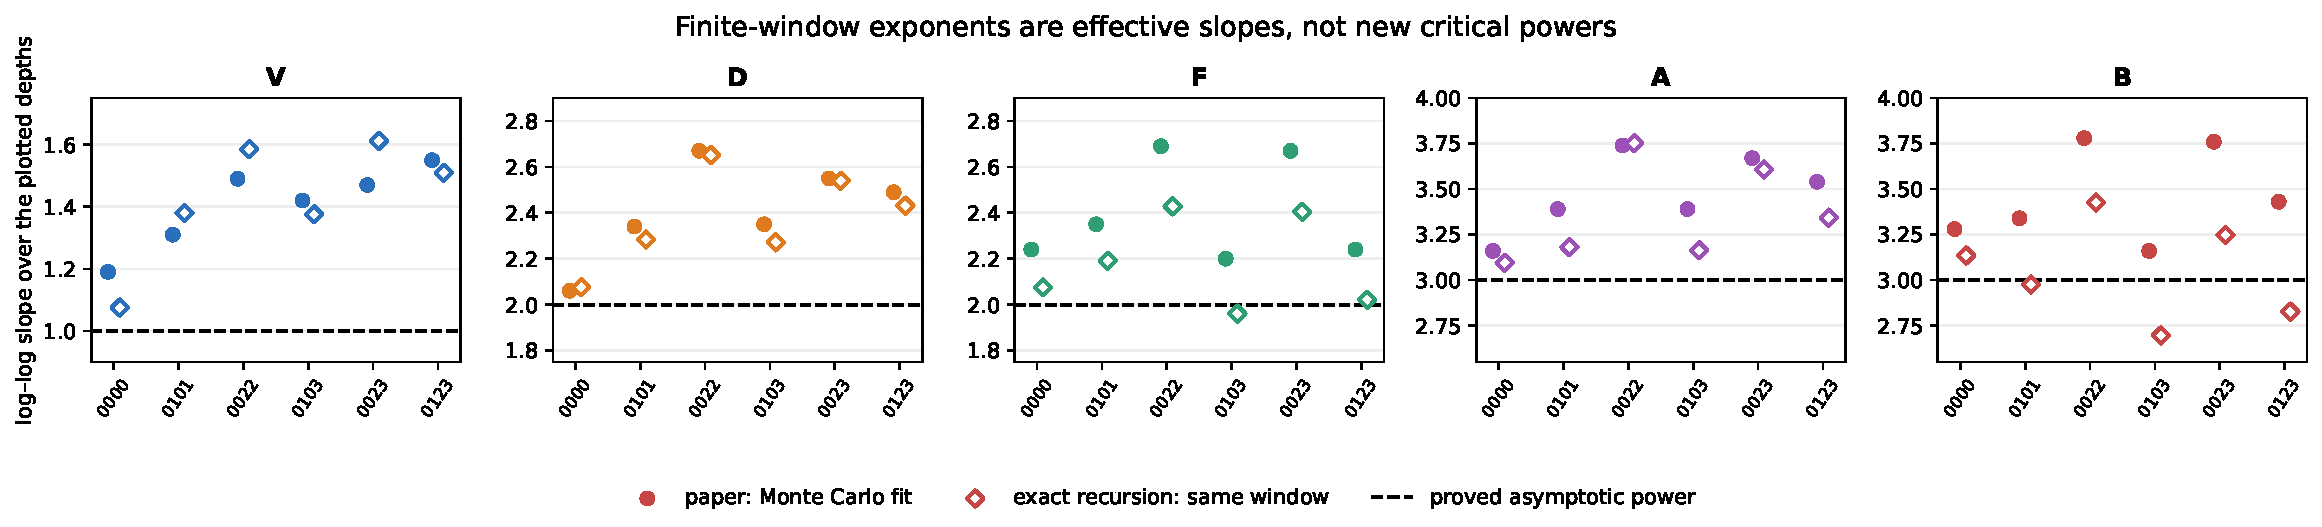
\includegraphics[width=\linewidth]{../../data/feynman/paper_exponent_comparison/paper_vs_exact_recursion_exponents.pdf}
\caption{The published Monte Carlo regression slopes, the deterministic
leading-width recursion under the same finite windows, and the proved
asymptotic powers.}
\label{fig:effective-slopes}
\end{figure}

\begin{figure}[t]
\centering
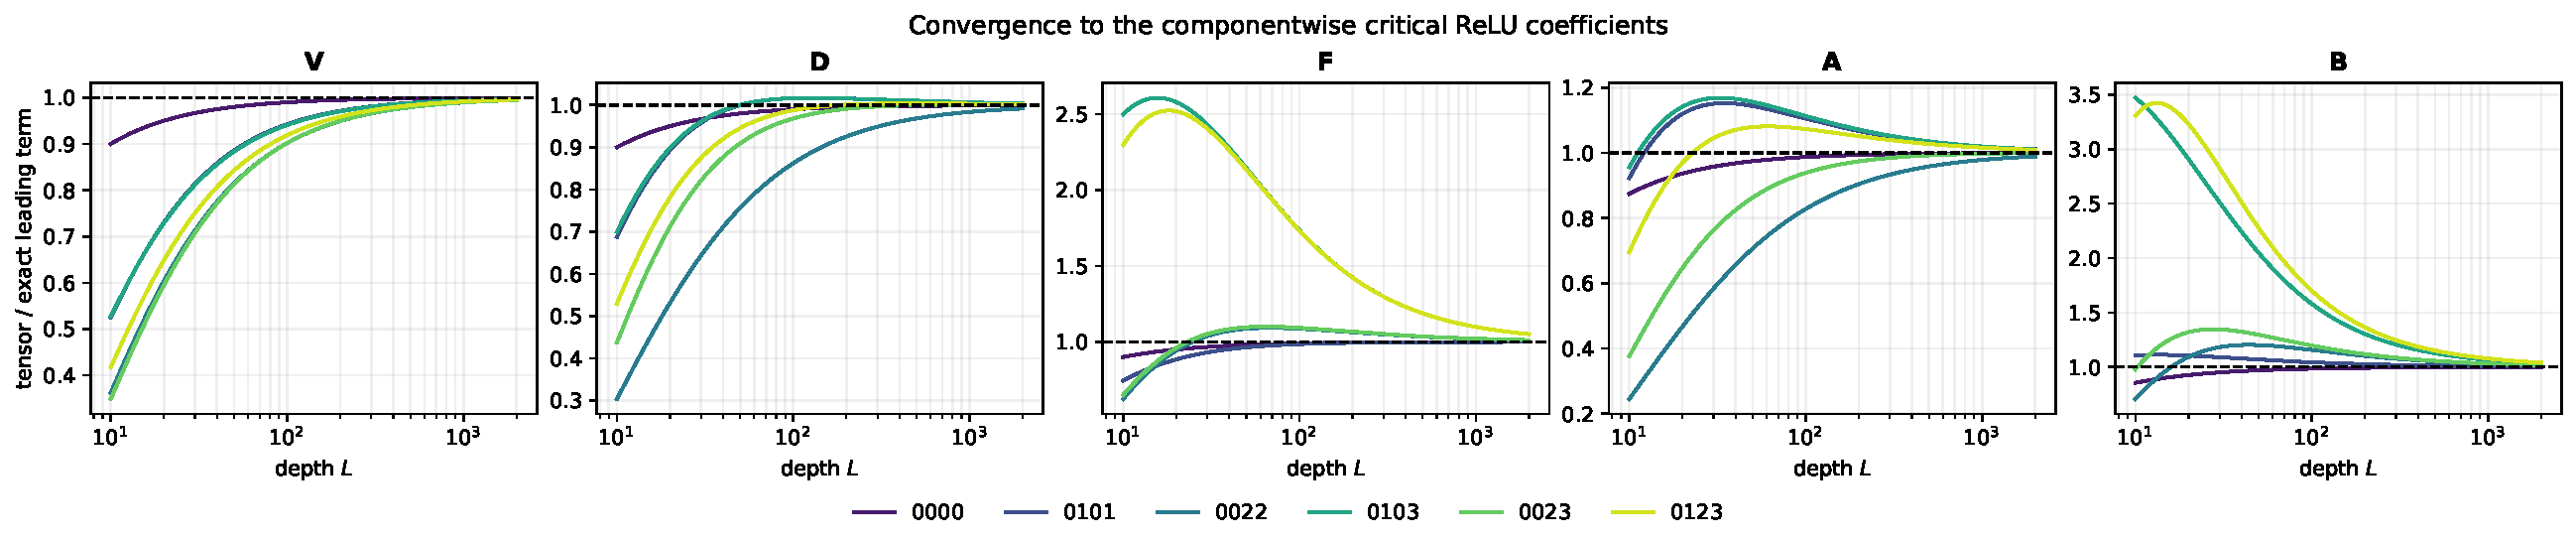
\includegraphics[width=\linewidth]{../../data/feynman/relu_tensor_asymptotics/relu_tensor_leading_coefficients.pdf}
\caption{Each component divided by its exact leading term from Theorem
\ref{thm:componentwise-powers}.  Slow, nonmonotone convergence explains why
depth \(30\) produces noninteger effective slopes.}
\label{fig:coefficient-convergence}
\end{figure}

\section{All-valence low-rank calculus}
\label{sec:weingarten}

We now compute the rank vertices exactly.  Let \(\cP_2(2k)\) denote the
perfect matchings of \(\{1,\ldots,2k\}\), and let
\(\tau=(1,2)(3,4)\cdots(2k-1,2k)\) pair the two legs belonging to each Gram
entry.  For a pairing \(\pi\), write \(\delta_I^\pi\) for the product of
Kronecker deltas identifying external row indices along \(\pi\), and
\(c(\pi\vee\tau)\) for the number of connected components of the graph formed
by the two matchings.

\subsection{The actual Gaussian MMNN vertex}

Let \(X\in\R^{n\times r}\) have iid standard-normal entries and
\(G=XX^\top/r\).  The following theorem is both the exact moment rule and a
complete connected Feynman rule.

\begin{theorem}[Gaussian Gram Wick rule]
\label{thm:gram-wick}
For arbitrary fixed \(k\) and concrete external indices
\(I=(i_1,j_1,\ldots,i_k,j_k)\),
\begin{align}
\E\prod_{t=1}^kG_{i_tj_t}
&=\sum_{\pi\in\cP_2(2k)}
\delta_I^\pi r^{c(\pi\vee\tau)-k},
\label{eq:gram-moment}\\
\cum(G_{i_1j_1},\ldots,G_{i_kj_k})
&=r^{1-k}
\sum_{\substack{\pi\in\cP_2(2k)\\c(\pi\vee\tau)=1}}
\delta_I^\pi.
\label{eq:gram-cumulant}
\end{align}
The formulas are finite-\(r\) identities, not asymptotic expansions.
\end{theorem}

In particular,
\begin{align}
\E G_{ij}&=\delta_{ij},\label{eq:gram-mean}\\
\Cov(G_{ij},G_{kl})
&=\frac1r(\delta_{ik}\delta_{jl}+\delta_{il}\delta_{jk}),
\label{eq:gram-cov}\\
\cum_k(G_{11})&=\frac{2^{k-1}(k-1)!}{r^{k-1}}.
\label{eq:gram-diag-cumulant}
\end{align}
Thus the rank expansion is controlled at every valence, including its
non-Gaussian corrections.  Equation \eqref{eq:gram-cumulant} is especially
useful computationally: a cumulant is obtained by retaining only connected
pairing diagrams.

\subsection{Whitened orientation and orthogonal Weingarten calculus}

Let \(U\in\R^{n\times r}\) be Haar on the Stiefel manifold
\(U^\top U=I_r\), and set \(P=UU^\top\), \(G=(n/r)P\).  For
\(\pi,\sigma\in\cP_2(2k)\), define the orthogonal Gram matrix
\begin{equation}
\mathcal G^{O(n)}_{\pi\sigma}=n^{c(\pi\vee\sigma)},
\qquad
\mathrm{Wg}^{O}_n=(\mathcal G^{O(n)})^{-1}.
\label{eq:orthogonal-wg}
\end{equation}

\begin{theorem}[All-valence Haar-projector rule]
\label{thm:projector-weingarten}
For arbitrary fixed \(k\) for which the orthogonal Gram matrix
\eqref{eq:orthogonal-wg} is invertible (in particular, \(n\ge k\)),
\begin{equation}
\E\prod_{t=1}^kG_{i_tj_t}
=\left(\frac nr\right)^k
\sum_{\pi,\sigma\in\cP_2(2k)}
\delta_I^\pi\,\mathrm{Wg}^{O}_n(\pi,\sigma)
r^{c(\sigma\vee\tau)}.
\label{eq:projector-moment}
\end{equation}
Joint cumulants follow by exact M\"obius inversion on set partitions.
At \(r=n\), \(G=I_n\) pathwise and every centered cumulant vanishes exactly.
\end{theorem}

\begin{corollary}[Exact full-rank endpoint]
\label{cor:full-rank-endpoint}
For the Stiefel-whitened model at \(r=n\), \(G=I_n\) pathwise.  Hence every
connected rank vertex of valence at least two vanishes, and the rank-colored
diagrammatics reduces to the dense Euclidean tangent calculus.  Equivalently,
\(M=UA\) is an orthogonal reparameterization of a dense trainable matrix.
For an iid Gaussian square \(W\), the function parameterization is full rank
almost surely but its Euclidean NTK is not this endpoint: the Wishart radial
vertices of \(WW^\top/n\) remain.
\end{corollary}

At second order, Theorem \ref{thm:projector-weingarten} gives
\begin{equation}
\Cov(G_{ij},G_{kl})
=\gamma_{n,r}
\left(\delta_{ik}\delta_{jl}+\delta_{il}\delta_{jk}
-\frac2n\delta_{ij}\delta_{kl}\right),
\label{eq:projector-covariance}
\end{equation}
with \(\gamma_{n,r}\) from \eqref{eq:gamma}.  For example,
\begin{align}
\Var(G_{11})&=\frac{2(n-r)}{r(n+2)},\\
\cum_3(G_{11})&=\frac{8(n-r)(n-2r)}{r^2(n+2)(n+4)}.
\end{align}
Our symbolic implementation constructs \(\mathrm{Wg}^{O}_n\) by exact
SymPy inversion, compresses coefficients by orthogonal coset type, and checks
diagonal moments against the beta law
\begin{equation}
\E G_{11}^k=\left(\frac nr\right)^k
\frac{(r/2)_k}{(n/2)_k}.
\end{equation}

\begin{remark}[Why both theorems are needed]
For Gaussian \(X=QR\), the Stiefel orientation \(Q\) is independent of the
Wishart radial factor \(R\), and
\[
XX^\top/r=Q(RR^\top/r)Q^\top.
\]
Theorem \ref{thm:projector-weingarten} integrates the orientation exactly;
Theorem \ref{thm:gram-wick} integrates orientation and radius together.  The
projector-only surrogate amounts to replacing \(RR^\top/r\) by a scalar
identity.  This is a change of tangent metric, not a harmless rewriting of the
Euclidean MMNN.
\end{remark}

\section{MMNN analogues and their exact depth exponents}
\label{sec:mmnn-exponents}

We now lift the definitions
\eqref{eq:original-V-definition}--\eqref{eq:original-AB-definition}, rather
than merely reusing their names.  For component indices \(a,b,c,d\in[r_\ell]\),
define the full (not \(1/n\)-stripped) MMNN tensors by
\begin{align}
\cum(h^a_1,h^b_2,h^c_3,h^d_4)
={}&\delta_{ab}\delta_{cd}\mathcal V_{1234}
+\delta_{ac}\delta_{bd}\mathcal V_{1324}
+\delta_{ad}\delta_{bc}\mathcal V_{1423},
\label{eq:mmnn-V-definition}\\
\cum(h^a_1,h^b_2,\Delta\Theta^{cd}_{34})
={}&\delta_{ab}\delta_{cd}\mathcal D_{1234}
+\delta_{ac}\delta_{bd}\mathcal F_{1324}
+\delta_{ad}\delta_{bc}\mathcal F_{1423},
\label{eq:mmnn-DF-definition}\\
\cum(\Delta\Theta^{ab}_{12},\Delta\Theta^{cd}_{34})
={}&\delta_{ab}\delta_{cd}\mathcal A_{1234}
+\delta_{ac}\delta_{bd}\mathcal B_{1324}
+\delta_{ad}\delta_{bc}\mathcal B_{1423}.
\label{eq:mmnn-AB-definition}
\end{align}
These decompositions follow from orthogonal invariance of the Gaussian
component initialization.  They are the literal MMNN counterparts of the
five non-MMNN tensors, with \(h^a\) replacing a dense neural channel and the
matrix NTK from \eqref{eq:pathwise-ntk} replacing the scalar-channel NTK.

For homogeneous widths \(n_\ell=n\) and ranks \(r_\ell=r\), each tensor has a
two-color connected expansion
\begin{equation}
\mathcal T_L=\frac1nT_L^{[n]}+\frac1rT_L^{[r]}
+O_{L}(n^{-2}+n^{-1}r^{-1}+r^{-2}),
\qquad
\mathcal T\in\{\mathcal V,\mathcal D,\mathcal F,\mathcal A,\mathcal B\}.
\label{eq:mmnn-colored-expansion}
\end{equation}
The blue coefficient \(T^{[n]}\) contains one connected empirical-feature
vertex; the red coefficient \(T^{[r]}\) contains one connected Gram vertex.
Mixed blue--red graphs start one order later.  In the Stiefel-whitened model,
\(r^{-1}T^{[r]}\) in \eqref{eq:mmnn-colored-expansion} is replaced by
\(\gamma_{n,r}T^{[S]}\), with the trace subtraction in
\eqref{eq:projector-covariance} included in \(T^{[S]}\).

The rank coefficients are computable without fitting.  Let
\(\mathfrak D_{T,\ell}^{ij;kl}\) denote the two-Gram-leg Fr\'echet derivative
obtained by differentiating the pathwise update \eqref{eq:pathwise-ntk} and
the corresponding activation moment defining \(T\).  The one-rank-vertex
source is exactly
\begin{align}
S_{T,\ell}^{[r]}
&=\sum_{ij,kl}\mathfrak D_{T,\ell}^{ij;kl}
(\delta_{ik}\delta_{jl}+\delta_{il}\delta_{jk}),
\label{eq:gaussian-rank-source}\\
S_{T,\ell}^{[S]}
&=\sum_{ij,kl}\mathfrak D_{T,\ell}^{ij;kl}
\left(\delta_{ik}\delta_{jl}+\delta_{il}\delta_{jk}
-\frac2n\delta_{ij}\delta_{kl}\right).
\label{eq:stiefel-rank-source}
\end{align}
Equations \eqref{eq:gaussian-rank-source} and
\eqref{eq:stiefel-rank-source} are respectively the coefficients of \(1/r\)
and \(\gamma_{n,r}\); all higher-valence sources follow from Theorems
\ref{thm:gram-wick} and \ref{thm:projector-weingarten}.  Thus Wick or
Weingarten calculus computes the amplitude tensor, including its index
dependence, rather than guessing it from a scalar rank count.

At first connected order, differentiation of the pathwise recursion gives
the triangular transported hierarchy, separately for
\(c\in\{[n],[r],[S]\}\),
\begin{align}
V^{c}_{\ell+1}&=\mathcal L_{V,\ell}V^c_\ell+S^c_{V,\ell},
\label{eq:mmnn-V-hierarchy}\\
C^{c}_{\ell+1}&=\mathcal L_{C,\ell}C^c_\ell
+\mathcal M_{CV,\ell}V^c_\ell+S^c_{C,\ell},
\qquad C=(D,F),
\label{eq:mmnn-C-hierarchy}\\
N^{c}_{\ell+1}&=\mathcal L_{N,\ell}N^c_\ell
+\mathcal M_{NC,\ell}C^c_\ell
+\mathcal M_{NV,\ell}V^c_\ell+S^c_{N,\ell},
\qquad N=(A,B).
\label{eq:mmnn-N-hierarchy}
\end{align}
All operators here are explicit Gaussian activation expectations.  In the
dense-compatible bias-free normalization, the blue specialization is
exactly \eqref{eq:V-rec}--\eqref{eq:B-rec}.  Retaining the trainable component
bias \(c_\ell\) adds a local identity source but does not alter the transport
powers below.

\begin{theorem}[MMNN two-color depth powers]
\label{thm:mmnn-powers}
Consider critical ReLU MMNNs and a fixed finite, non-collinear input set.
Let \(n=n(L)\), \(r=r(L)\) tend to infinity with
\(n/r\to\rho\in(0,\infty)\), and put
\(\epsilon_{n,r}=n^{-1}+r^{-1}\).  Uniformly in the perturbative depth window
\(L^3\epsilon_{n,r}\to0\), the tensors
\eqref{eq:mmnn-V-definition}--\eqref{eq:mmnn-AB-definition} obey
\begin{align}
\mathcal V_L&=L\left(\frac{v^{[n]}}n+\frac{v^{[r]}}r+o(\epsilon_{n,r})\right),
\label{eq:mmnn-V-power}\\
(\mathcal D_L,\mathcal F_L)
&=L^2\left(\frac{(d^{[n]},f^{[n]})}n
+\frac{(d^{[r]},f^{[r]})}r+o(\epsilon_{n,r})\right),
\label{eq:mmnn-DF-power}\\
(\mathcal A_L,\mathcal B_L)
&=L^3\left(\frac{(a^{[n]},b^{[n]})}n
+\frac{(a^{[r]},b^{[r]})}r+o(\epsilon_{n,r})\right).
\label{eq:mmnn-AB-power}
\end{align}
The same statement holds for the whitened Stiefel model after replacing
\(r^{-1}t^{[r]}\) by \(\gamma_{n,r}t^{[S]}\).  The blue coefficients are
strictly nonzero componentwise and, in the dense-compatible normalization,
equal the coefficients in Theorem \ref{thm:componentwise-powers}; hence all
five displayed powers are attained.  In a pure-rank limit \(n/r\to\infty\),
the stated powers remain upper bounds and are attained precisely in sectors
where the corresponding projected source
\eqref{eq:gaussian-rank-source} is nonzero.
\end{theorem}

\begin{proof}
At first connected order a diagram contains exactly one blue or one red
connected vertex; this proves the additive decomposition
\eqref{eq:mmnn-colored-expansion}.  Conditioning on the preceding layer and
applying the law of total cumulance gives
\eqref{eq:mmnn-V-hierarchy}--\eqref{eq:mmnn-N-hierarchy}.  The conditional
blue cumulant is the ordinary empirical-average cumulant, whereas the red
conditional cumulant is \eqref{eq:gram-cov}; this proves
\eqref{eq:gaussian-rank-source}.  Equation
\eqref{eq:stiefel-rank-source} follows identically from
\eqref{eq:projector-covariance}.

By Lemma \ref{lem:critical-drift}, the critical gate transport has the form
\(I+\mathcal K/L+O(\log L/L^2)\).  The local source in the \(V\) block is
\(O(1)\); the mixed block has one possible NTK path and source \(O(L)\); the
NTK-covariance block has two such paths and source \(O(L^2)\).  The collision
generators are finite dimensional and have eigenvalues \(0,-3,-6\).
Applying the discrete transport limit
\eqref{eq:discrete-transport-limit} with \(p=1,2,3\) yields respectively
\(L,L^2,L^3\).  More explicitly, for each color and block,
\begin{equation}
t_T^c=(p_T I-\mathcal K_T)^{-1}s_T^c,
\qquad
(p_V,p_D,p_F,p_A,p_B)=(1,2,2,3,3),
\label{eq:mmnn-leading-coefficient}
\end{equation}
where \(s_T^c\) is the collision limit of the exact source above.  This is an
exact finite-dimensional computation of every leading amplitude.

A diagram with at least two connected vertices is smaller by another factor
\(\epsilon_{n,r}\); its worst secular growth relative to first order is
\(O(L^3\epsilon_{n,r})\).  The stated depth-window condition therefore makes
their sum negligible.  Finally, the blue dense-compatible source reduces to
the non-MMNN recursion and its coefficients are strictly positive by Theorem
\ref{thm:componentwise-powers}, proving attainment.  If the blue sector is
removed asymptotically, the same argument proves the claimed source-projection
criterion for the red sector.
\end{proof}

\begin{table}[t]
\centering
\caption{Exact critical depth exponents.  The dense column gives the physical
connected cumulant, not the \(1/n\)-stripped coefficient.  Constants and
sample-index contractions are suppressed.}
\label{tab:dense-mmnn-exponents}
\small
\begin{tabular}{lcccc}
\toprule
tensor sector & exponent & dense/non-MMNN & Gaussian MMNN & Stiefel MMNN\\
\midrule
\(V\) & \(1\) & \(L/n\) & \(L(1/n+1/r)\) & \(L(1/n+\gamma_{n,r})\)\\
\(D,F\) & \(2\) & \(L^2/n\) & \(L^2(1/n+1/r)\) & \(L^2(1/n+\gamma_{n,r})\)\\
\(A,B\) & \(3\) & \(L^3/n\) & \(L^3(1/n+1/r)\) & \(L^3(1/n+\gamma_{n,r})\)\\
\bottomrule
\end{tabular}
\end{table}

Table \ref{tab:dense-mmnn-exponents} is the requested separation.  Equal
depth powers do not mean equal theories: MMNNs have an additional rank
amplitude, mixed higher-order diagrams, and a different breakdown scale.  At
\(r=n\), the Stiefel rank amplitude vanishes exactly and the dense tangent
theory is recovered.  At \(r=n\) with an iid Gaussian frozen factor, the
Wishart radial amplitude remains; full matrix rank alone therefore does not
recover the dense Euclidean NTK.

\section{Benigni--Paquette blocks and multilayer concatenation}
\label{sec:bp-concatenation}

The preceding Feynman calculation controls finite-width and finite-rank
deviations at fixed sample size.  The quadratic sample--parameter regime of
Benigni and Paquette \citep{BenigniPaquette2025} supplies a complementary,
nonperturbative bulk
law.  We now connect the two without identifying a two-layer network with an
entire deep network.

For a unit output direction \(u\in\R^{r_L}\), let
\begin{equation}
P_{\ell\to L}(x)=J_L(x)J_{L-1}(x)\cdots J_{\ell+1}(x),
\qquad P_{L\to L}=I.
\label{eq:downstream-transport}
\end{equation}
Define the tangent feature born at layer \(\ell\) by
\begin{equation}
\omega_{\ell,u}(x)=
\begin{bmatrix}
n_\ell^{-1/2}\phi(z_\ell(x))\otimes P_{\ell\to L}(x)^\top u\\
P_{\ell\to L}(x)^\top u
\end{bmatrix}
\in\R^{r_\ell(n_\ell+1)},
\qquad
\omega_{L,u}(x)=\bigoplus_{\ell=1}^L\omega_{\ell,u}(x).
\label{eq:concatenated-tangent-feature}
\end{equation}
The second entry records the trainable component bias and is omitted in the
bias-free model.

\begin{proposition}[Exact concatenated Gram representation]
\label{prop:concatenated-gram}
For every finite MMNN realization and all inputs \(x,y\),
\begin{equation}
u^\top\Theta_L(x,y)u
=\langle\omega_{L,u}(x),\omega_{L,u}(y)\rangle.
\label{eq:mmnn-concatenated-gram}
\end{equation}
Consequently the scalar-output sample NTK on \(N\) inputs is the Gram matrix
of a concatenation of \(L\) low-rank tangent blocks, with total tangent
dimension
\begin{equation}
d_L=\sum_{\ell=1}^L r_\ell(n_\ell+1).
\label{eq:total-tangent-dimension}
\end{equation}
\end{proposition}

\begin{proof}
The derivative with respect to one entry of the trainable right factor is
\[
\frac{\partial\,u^\top h_L(x)}{\partial(A_\ell)_{a\mu}}
=\frac{\phi(z_{\ell,\mu}(x))}{\sqrt{n_\ell}}\,
u^\top P_{\ell\to L}(x)e_a,
\]
whereas differentiation with respect to \(c_\ell^a\) gives
\(u^\top P_{\ell\to L}(x)e_a\).  Taking the Euclidean inner product over
\((a,\mu)\), then summing over \(\ell\), proves
\eqref{eq:mmnn-concatenated-gram}.  This is also the iterated form of the
pathwise recursion \eqref{eq:pathwise-ntk}.
\end{proof}

For one two-layer block, the tangent row of Benigni and Paquette
\citep{BenigniPaquette2025} is
\begin{equation}
\omega_{\rm BP}(x)
=x\otimes D\phi(x^\top W/\sqrt d)\in\R^{dp};
\label{eq:bp-tangent-row}
\end{equation}
its normalized Gram matrix is exactly
\[
\frac{XX^\top}{d}\odot
\frac{\phi(XW/\sqrt d)D^2\phi(XW/\sqrt d)^\top}{p}.
\]
Equation \eqref{eq:concatenated-tangent-feature} has the same Kronecker-Gram
form, with \(P_{\ell\to L}^\top u\) playing the transported-gain role of the
weighted derivative features.  The identification is exact algebraically;
the probabilistic assumptions of the two-layer theorem must still be checked
for the transported features.

Let \(x_1,\ldots,x_N\) be iid data and condition on all network matrices.
The rows \(\omega_{L,u}(x_i)\) are then iid.  Center them, put
\[
\xi_L(x)=\sqrt{d_L}\,[\omega_{L,u}(x)
-\E_x\omega_{L,u}(x)],
\qquad
\mathcal Q_L=\E_x[\xi_L(x)\xi_L(x)^\top\mid\{W,A\}],
\]
and let \(\pi_L\) be the limiting empirical eigenvalue distribution of the
block population covariance \(\mathcal Q_L\).

\begin{theorem}[Conditional multilayer Marchenko--Pastur law]
\label{thm:mmnn-bp-law}
Suppose \(N/d_L\to\gamma\in(0,\infty)\), the empirical law of
\(\mathcal Q_L\) converges in probability to a deterministic compactly
supported law \(\pi_L\), its operator norm is tight, and the centered tangent
rows satisfy the Bai--Zhou quadratic-form concentration condition.  Then the
empirical spectral distribution of the centered MMNN sample NTK converges in
probability to
\begin{equation}
\mu_L=\mu_{\rm MP}^{\gamma}\boxtimes\pi_L.
\label{eq:mmnn-bp-law}
\end{equation}
The discarded conditional mean changes the sample Gram matrix by rank at
most two and therefore does not change its limiting bulk law.
\end{theorem}

\begin{proof}
By Proposition \ref{prop:concatenated-gram}, the centered sample NTK is
\(d_L^{-1}\Xi_L\Xi_L^\top\), where the rows of \(\Xi_L\) are conditionally
iid with covariance \(\mathcal Q_L\).  The Bai--Zhou sample-covariance
theorem, in the form used by Benigni and Paquette
\citep{BenigniPaquette2025}, gives
\eqref{eq:mmnn-bp-law}.  Centering a Gram matrix changes it by the sum of two
rank-one cross terms and one rank-one mean term, whose total rank is at most
two.
\end{proof}

The new multilayer content is therefore the population covariance
\(\mathcal Q_L\), not a second application of the MP map.  It is a block
matrix
\begin{equation}
\mathcal Q_L=(\mathcal Q_{\ell k})_{\ell,k\le L},
\qquad
\mathcal Q_{\ell k}
=d_L\Cov_x(\omega_{\ell,u}(x),\omega_{k,u}(x)\mid\{W,A\}).
\label{eq:bp-block-covariance}
\end{equation}
The diagonal blocks are transported Benigni--Paquette covariance tensors.
The off-diagonal blocks record correlations between tangent features born at
different depths and are computed by the same colored Feynman rules as
\eqref{eq:mmnn-V-hierarchy}--\eqref{eq:mmnn-N-hierarchy}.

If the off-diagonal blocks are negligible in normalized Hilbert--Schmidt
norm, write \(d_\ell=r_\ell(n_\ell+1)\) and
\(\alpha_\ell=d_\ell/d_L\).  If the naturally normalized diagonal block has
limiting law \(\pi_\ell^{\rm BP}\), then
\begin{equation}
\pi_L=\sum_{\ell=1}^L
\alpha_\ell\,(\alpha_\ell^{-1}\cdot)_\#\pi_\ell^{\rm BP},
\qquad
\mu_L=\mu_{\rm MP}^{\gamma}\boxtimes\pi_L.
\label{eq:bp-decoupled-mixture}
\end{equation}
When cross-layer blocks persist, their full block law must be retained;
replacing it by a free additive convolution is an additional asymptotic
freeness hypothesis, not a consequence of concatenation alone.

\begin{corollary}[Closed homogeneous concatenation law]
\label{cor:bp-homogeneous-concatenation}
Assume the hypotheses of Theorem \ref{thm:mmnn-bp-law}, negligible
off-diagonal population blocks, and \(L\) statistically identical tangent
blocks of dimension \(d p\).  If
\(N/(dp)\to\gamma_1\) and the one-block population covariance law is
\(\mu_{\nu,\varphi}\) in the notation of Benigni and Paquette, then
\begin{equation}
\boxed{\quad
\mu_{\Theta_L}
=\mu_{\rm MP}^{\gamma_1/L}\boxtimes
(L\cdot)_\#\mu_{\nu,\varphi}.
\quad}
\label{eq:bp-homogeneous-spectrum}
\end{equation}
More generally, for transported squared gains \(\tau_\ell^2\) and possibly
different one-block laws,
\begin{equation}
\mu_{\Theta_L}
=\mu_{\rm MP}^{\gamma_1/L}\boxtimes
\left[\frac1L\sum_{\ell=1}^L
(L\tau_\ell^2\cdot)_\#\mu_{\nu_\ell,\varphi_\ell}\right].
\label{eq:bp-inhomogeneous-spectrum}
\end{equation}
In the explicit Benigni--Paquette case \(\nu=\delta_1\) or
\(\varphi(x)=ax+b\),
\begin{equation}
\mu_{\nu,\varphi}
=\operatorname{Law}(\alpha_\varphi^2\chi+\beta_\psi^2),
\label{eq:bp-explicit-population}
\end{equation}
where
\begin{align}
\operatorname{Law}(\chi)
={}&\frac{\gamma_2}{2}
(\mu_{\rm MP}^{\gamma_2}\boxtimes\nu)
*(\mu_{\rm MP}^{\gamma_2}\boxtimes\nu)
\nonumber\\
&+(1-\gamma_2)(\mu_{\rm MP}^{\gamma_2}\boxtimes\nu)
+\frac{\gamma_2}{2}\delta_0.
\label{eq:bp-chi-law}
\end{align}
Equations \eqref{eq:bp-homogeneous-spectrum} and \eqref{eq:bp-chi-law}
therefore compute the concatenated Gram--NTK bulk using only scalar measure
operations and the MP fixed point.
\end{corollary}

\begin{proof}
Here \(d_L=Ldp\), hence \(N/d_L\to\gamma_1/L\) and
\(\alpha_\ell=1/L\).  Equation \eqref{eq:bp-decoupled-mixture} gives
\(\pi_L=(L\cdot)_\#\mu_{\nu,\varphi}\) in the homogeneous unit-gain case and
the mixture in \eqref{eq:bp-inhomogeneous-spectrum} otherwise.  Theorem
\ref{thm:mmnn-bp-law} supplies the outer MP map.  The last statement is the
explicit population law of Benigni and Paquette.
\end{proof}

\subsection{Spectral deviations around the quadratic-scaling bulk}

The Benigni--Paquette law can be used as the base spectrum rather than
replaced by a Wigner base.  Let \(s(z)\) be the Stieltjes transform of
\(\mu_{\rm MP}^{\gamma}\boxtimes\pi\), so that
\begin{equation}
s(z)=\int\frac{\dd\pi(t)}
{t[1-\gamma(1+zs(z))]-z}.
\label{eq:bp-mp-fixed-point}
\end{equation}
Put \(a(z)=1-\gamma(1+zs(z))\) and
\(D(t,z)=ta(z)-z\).  For a signed population-law perturbation
\(\delta\pi\) of total mass zero, differentiation of
\eqref{eq:bp-mp-fixed-point} gives the exact linear response
\begin{equation}
\delta s(z)=
\frac{\displaystyle\int D(t,z)^{-1}\dd(\delta\pi)(t)}
{\displaystyle 1-\gamma z\int tD(t,z)^{-2}\dd\pi(t)}.
\label{eq:bp-linear-response}
\end{equation}
Thus width- and rank-colored diagrams first perturb the block covariance law
\(\pi_L\); equation \eqref{eq:bp-linear-response} propagates that perturbation
to the bulk density
\(\delta\rho(\lambda)=\pi^{-1}\Im\delta s(\lambda+i0)\).

\begin{figure}[t]
\centering
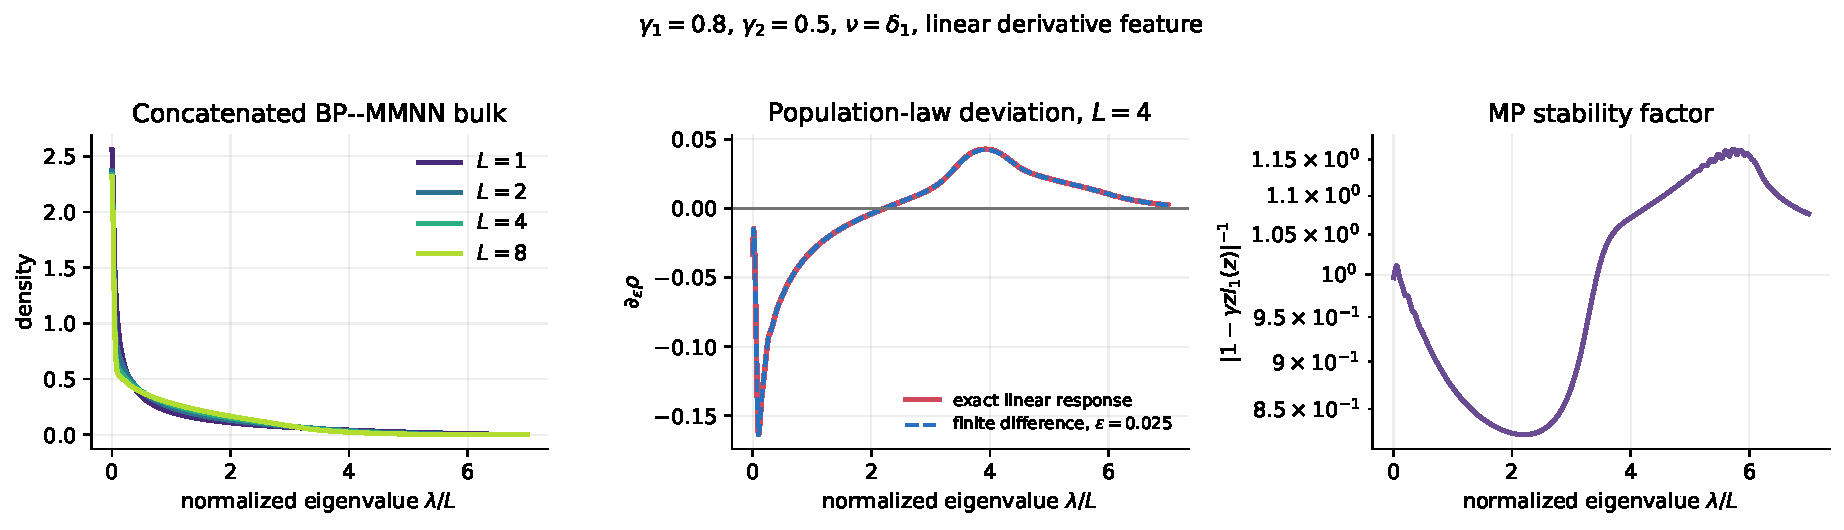
\includegraphics[width=\linewidth]{../../data/feynman/benigni_paquette_mmnn_spectrum/benigni_paquette_mmnn_spectrum.pdf}
\caption{Conditional exact quadratic-scaling spectrum for homogeneous
concatenated Benigni--Paquette tangent blocks.  Left: the normalized spectrum
from \eqref{eq:bp-homogeneous-spectrum}.  Center: the analytic population-law
response \eqref{eq:bp-linear-response} and a finite difference.  Right: the
MP stability factor that filters a Feynman correction.  We use
\(\gamma_1=0.8\), \(\gamma_2=0.5\), \(\nu=\delta_1\), and the explicit linear
derivative-feature law.}
\label{fig:bp-mmnn-spectrum}
\end{figure}

Sample-to-sample spectral fluctuations retain the full tensor information.
If \(R_z=(K_{\rm BP}-zI)^{-1}\), the first resolvent variation is
\begin{equation}
\delta m_N(z)=-\frac1N\Tr(R_z\,\Delta K\,R_z),
\label{eq:bp-random-resolvent-response}
\end{equation}
and its covariance follows by contracting two copies of \(R_z^2\) with the
\(A/B\) tensor, including the additional \(1/r\) Gram or Weingarten vertex.
Consequently its perturbative scale is
\(L^3(1/n+1/r)\), while its spectral shape is filtered by the stability
denominator in \eqref{eq:bp-linear-response}.  Near a quadratic-scaling
spectral edge this denominator may be small, amplifying a diagrammatically
small finite-rank correction.

\begin{remark}[ReLU regularity]
\label{rem:bp-relu}
The theorem of Benigni and Paquette \citep{BenigniPaquette2025} assumes that
the derivative feature \(\phi=\sigma'\) is pseudo-Lipschitz.  The exact ReLU gate
\(\one_{x>0}\) is discontinuous and is not covered verbatim.  Equations
\eqref{eq:mmnn-concatenated-gram} and \eqref{eq:bp-block-covariance} remain
exact for ReLU, but the quadratic-scaling limit then requires either a
smoothed gate followed by a uniform limit or a separate universality proof.
\end{remark}

\section{Neural quadratic forms as an exact Landau resummation}
\label{sec:nqf}

We now integrate the neural quadratic form (NQF) of
Liu Ziyin et al.~\citep{NQF2026} with the preceding finite-width and
finite-rank diagrams.
To prevent a serious notation collision, throughout this section
\(\mathscr A_x\in\R^{p\times p}\) denotes the NQF \emph{structure matrix},
\(\mathsf M=WW^\top\) denotes its dynamic order parameter, and
\(\mathcal A_{abcd},\mathcal B_{abcd}\) continue to denote the four-sample
NTK-covariance tensors of Section~\ref{sec:mmnn-exponents}.  The frozen MMNN
metric \(G=XX^\top/r\) is yet another Gram matrix.  Algebraically, \(G\) and
\(\mathsf M\) have the same double-line indices; dynamically they have
different roles: \(G\) is quenched, while \(\mathsf M(t)\) is trained.

\subsection{Symmetry, the normal form, and the MMNN dictionary}

Let \(W=(w_1,\ldots,w_d)\in\R^{p\times d}\) collect exchangeable components.
The zero-gradient-at-zero (ZGZ) condition of Liu Ziyin et
al.~\citep{NQF2026} is
\begin{equation}
\nabla_{w_i}f_x(w_1,\ldots,w_d)\big|_{w_i=0}=0
\quad\hbox{for every value of the other components.}
\label{eq:zgz}
\end{equation}

\begin{proposition}[Symmetry-derived local vertex]
\label{prop:nqf-normal-form}
If \(f_x\) is \(C^3\), invariant under \(S_d\), and satisfies
\eqref{eq:zgz}, then, locally at the symmetric origin,
\begin{equation}
f_x(W)=f_x(0)+\Tr(\mathsf M\mathscr A_x)+R_{3,x}(W),
\qquad \mathsf M=WW^\top,
\qquad |R_{3,x}(W)|\le C_x\|W\|^3.
\label{eq:nqf-local-form}
\end{equation}
If each component also has an independent sign symmetry
\(w_i\mapsto-w_i\), the remainder is \(O(\|W\|^4)\).  Without ZGZ the
complete quadratic normal form is
\begin{equation}
f_x(W)=f_x(0)+g_x^\top\mu+\mu^\top\mathscr B_x\mu
+\Tr(\mathsf M\mathscr A_x)+O(\|W\|^3),
\qquad \mu=W\one.
\label{eq:nqf-general-form}
\end{equation}
\end{proposition}

\begin{proof}
Write the Taylor Hessian in \(p\times p\) blocks \(H_{ij}\).  Permutation
symmetry makes all first derivatives equal, all diagonal blocks equal, and
all off-diagonal blocks equal.  Because the left-hand side of
\eqref{eq:zgz} is identically zero as a function of the other components,
the common first derivative and every mixed block \(H_{ij}\), \(i\ne j\),
vanish.  Setting \(\mathscr A_x=H_{ii}/2\) leaves
\(\frac12\sum_iw_i^\top H_{ii}w_i=\Tr(WW^\top\mathscr A_x)\).
Taylor's theorem with locally bounded third derivative gives the stated
remainder.  Independent sign symmetry eliminates every monomial containing
an odd power of a component, hence all cubic terms.  If ZGZ is removed, the
common first derivative gives \(g_x^\top\mu\), while the common mixed Hessian
can be rewritten as a quadratic form in \(\mu\) plus a redefinition of the
self-interaction matrix, which gives \eqref{eq:nqf-general-form}.
\end{proof}

The result is a Landau construction: \(S_d\) fixes the allowed invariant,
and the architecture fixes the coupling \(\mathscr A_x\).  It is essential
not to infer ZGZ merely from low rank.  Indeed, the one-block MMNN map
\(A_1\mapsto A_1\phi(W_1x)\) is exactly linear in its trainable right factor
and therefore occupies the \(g_x^\top\mu\) sector of
\eqref{eq:nqf-general-form}.  The pure quadratic sector first appears when
two trainable factors interact.

For example, consider two bias-free MMNN blocks, a scalar readout \(u\), a
smooth activation with \(\phi(0)=0\), and let
\(s_1(x)=\phi(W_1x/\sqrt{r_0})\).  At \((A_1,A_2)=(0,0)\),
\begin{equation}
u^\top h_2(x)=
\frac{\phi'(0)}{\sqrt{n_1n_2r_1}}
u^\top A_2W_2A_1s_1(x)
+O(\|(A_1,A_2)\|^3).
\label{eq:two-block-nqf}
\end{equation}
After vectorizing \(A_1,A_2\), the displayed bilinear form is
\(b^\top\mathscr C_xa\), hence it has structure matrix
\begin{equation}
\mathscr A_x=\frac12
\begin{bmatrix}0&\mathscr C_x^\top\\
\mathscr C_x&0\end{bmatrix}.
\label{eq:mmnn-nqf-structure}
\end{equation}
The frozen matrix \(W_2\) is part of \(\mathscr C_x\).  Contracting two
\(A_1\)-legs of \(\mathscr C_x\) produces precisely
\(G=W_2W_2^\top/r_1\); thus Theorems~\ref{thm:gram-wick} and
\ref{thm:projector-weingarten} compute the radial and orientation statistics
of the random Landau vertex.  For three or more simultaneously vanishing
right factors, the global leading degree is generally the number of blocks,
not two.  One must then either expand around a nonzero reference state or use
the layerwise deep NQF; a global quadratic claim would be false.

\subsection{Closed dynamics and the resummed dynamic NTK}

We first treat the pure ZGZ model as an exact model,
\begin{equation}
f_\mu(W)=\Tr(\mathsf M\mathscr A_\mu),\qquad
\mathcal L=\frac1m\sum_{\mu=1}^m(f_\mu-y_\mu)^2,
\label{eq:pure-nqf-loss}
\end{equation}
with symmetric \(\mathscr A_\mu\).  Define the structure-covariance operator
and target matrix
\begin{equation}
\mathscr K(X)=\frac4m\sum_{\mu=1}^m
\langle\mathscr A_\mu,X\rangle_F\mathscr A_\mu,
\qquad
Y=\frac4m\sum_{\mu=1}^my_\mu\mathscr A_\mu.
\label{eq:nqf-K-Y}
\end{equation}

\begin{theorem}[Exact quadratic-vertex resummation]
\label{thm:nqf-resummation}
For gradient flow in \eqref{eq:pure-nqf-loss},
\begin{align}
\dot W&=-H(\mathsf M)W,
&H(\mathsf M)&=\mathscr K(\mathsf M)-Y,
\label{eq:nqf-W-flow}\\
\dot{\mathsf M}
&=Y\mathsf M+\mathsf MY
-\mathscr K(\mathsf M)\mathsf M-\mathsf M\mathscr K(\mathsf M).
\label{eq:nqf-M-flow}
\end{align}
The empirical NTK is, at every finite \(p,d,m\),
\begin{equation}
\Theta_{\mu\nu}(t)
=4\Tr(\mathscr A_\mu\mathscr A_\nu\mathsf M(t)).
\label{eq:nqf-dynamic-ntk}
\end{equation}
Equations \eqref{eq:nqf-M-flow}--\eqref{eq:nqf-dynamic-ntk} resum every
chain made only of quadratic structure vertices.  No width or lazy-training
limit is used.
\end{theorem}

\begin{proof}
Since \(\nabla_Wf_\mu=2\mathscr A_\mu W\), direct differentiation of
\eqref{eq:pure-nqf-loss} gives
\(\dot W=-(4/m)\sum_\mu(f_\mu-y_\mu)\mathscr A_\mu W\), which is
\eqref{eq:nqf-W-flow}.  Applying the product rule to
\(\mathsf M=WW^\top\) proves \eqref{eq:nqf-M-flow}.  Finally,
\begin{align*}
\langle\nabla_Wf_\mu,\nabla_Wf_\nu\rangle_F
&=4\Tr(W^\top\mathscr A_\mu\mathscr A_\nu W)
=4\Tr(\mathscr A_\mu\mathscr A_\nu\mathsf M),
\end{align*}
which proves \eqref{eq:nqf-dynamic-ntk}.  The right side of the flow depends
on \(W\) only through \(\mathsf M\), so adding another two-leg insertion
cannot generate a new order parameter; induction over the number of
insertions proves the resummation statement.
\end{proof}

For general data the propagator
\(U(t)=\mathcal T\exp[-\int_0^tH(\mathsf M(s))\dd s]\) gives
\(\mathsf M(t)=U(t)\mathsf M(0)U(t)^\top\), but this is a self-consistent
time-ordered representation, not a scalar closed form.  A genuinely closed
noncommutative solution follows under the isotropic four-tensor identity
\begin{equation}
\frac1m\sum_\mu(\mathscr A_\mu)_{ij}(\mathscr A_\mu)_{kl}
=\frac c2(\delta_{ik}\delta_{jl}+\delta_{il}\delta_{jk}).
\label{eq:nqf-isotropy}
\end{equation}
Then \(\mathscr K(\mathsf M)=4c\mathsf M\), so
\begin{equation}
\dot{\mathsf M}=Y\mathsf M+\mathsf MY-8c\mathsf M^2,
\qquad
\mathsf M(t)=e^{Yt}\mathsf M_0
[I+8c\Phi(t)\mathsf M_0]^{-1}e^{Yt},
\quad
\Phi(t)=\int_0^te^{2Ys}\dd s.
\label{eq:nqf-isotropic-resummation}
\end{equation}
Substitution verifies the Riccati equation.  Diagrammatically,
\eqref{eq:nqf-isotropic-resummation} is an exact matrix rainbow sum, whereas
the deformed-Wigner Dyson equation of Section~\ref{sec:spectral} resums a
different object: ensemble fluctuations around a base kernel.

For completeness, the non-ZGZ quadratic model
\eqref{eq:nqf-general-form} also closes exactly, now on
\((\mu,\mathsf M)\).  With \(u_x=g_x+2\mathscr B_x\mu\), its NTK is
\begin{align}
\Theta(x,x')={}&d\,u_x^\top u_{x'}
+2u_x^\top\mathscr A_{x'}\mu
+2\mu^\top\mathscr A_xu_{x'}
+4\Tr(\mathscr A_x\mathscr A_{x'}\mathsf M).
\label{eq:nqf-general-ntk}
\end{align}
This formula is the correct one-block MMNN entry point because its linear
sector need not vanish.

The diagrammatic simplification can also be stated at all valences.  For a
matrix \(C\), write \(C_s=(C+C^\top)/2\) and
\(Q_C=\Tr(C\mathsf M)=\Tr(C_s\mathsf M)\).

\begin{proposition}[Exact NQF initialization vertices]
\label{prop:nqf-all-valence}
Let \(W_0=\sqrt{\epsilon/d}\,Z\), where the entries of
\(Z\in\R^{p\times d}\) are iid standard Gaussian.  For symmetric test
matrices \(C_1,\ldots,C_q\) and \(q\ge2\),
\begin{equation}
\cum(Q_{C_1},\ldots,Q_{C_q})
=\frac{2^{q-1}\epsilon^q}{d^{q-1}}
\sum_{\pi\in S_{q-1}}
\Tr(C_1C_{\pi(2)}\cdots C_{\pi(q)}).
\label{eq:nqf-gaussian-cumulants}
\end{equation}
Here \(S_{q-1}\) permutes \(\{2,\ldots,q\}\).  In particular,
\begin{align}
\Cov(f_\mu,f_\nu)
&=\frac{2\epsilon^2}{d}\Tr(\mathscr A_\mu\mathscr A_\nu),
\label{eq:nqf-output-covariance}\\
\Cov(\Theta_{\mu\nu},\Theta_{\rho\sigma})
&=\frac{32\epsilon^2}{d}
\Tr(C_{\mu\nu}C_{\rho\sigma}),
\quad
C_{\mu\nu}=\frac12(\mathscr A_\mu\mathscr A_\nu
+\mathscr A_\nu\mathscr A_\mu).
\label{eq:nqf-ntk-covariance}
\end{align}
Every joint \(V,D,F,A,B\)-type cumulant of NQF outputs and NTK entries is
obtained from \eqref{eq:nqf-gaussian-cumulants} by using
\(C=\mathscr A_\mu\) for an output and \(C=4C_{\mu\nu}\) for an NTK entry.
For \(\mathsf M_0=\epsilon(p/d)UU^\top\), the corresponding finite-
\((p,d)\) formula is exactly Theorem~\ref{thm:projector-weingarten} followed
by M\"obius inversion; all connected vertices vanish pathwise at \(d=p\).
\end{proposition}

\begin{proof}
Write \(Q_C=(\epsilon/d)\sum_{a=1}^d z_a^\top Cz_a\) with independent
\(z_a\sim N(0,I_p)\).  The logarithmic moment-generating function of
Gaussian quadratic forms is
\begin{equation*}
-\frac12\log\det\left(I-2\sum_{j=1}^qt_jC_j\right).
\end{equation*}
Expanding \(-\log\det(I-X)=\sum_{k\ge1}\Tr(X^k)/k\) and extracting
\(t_1\cdots t_q\) gives
\(2^{q-1}\sum_{\pi\in S_{q-1}}
\Tr(C_1C_{\pi(2)}\cdots C_{\pi(q)})\) for one column.  Cumulants add over
independent columns and scale homogeneously, proving
\eqref{eq:nqf-gaussian-cumulants}.  Equations
\eqref{eq:nqf-output-covariance} and
\eqref{eq:nqf-ntk-covariance} follow from
\eqref{eq:nqf-dynamic-ntk}.  The Stiefel claim is the projector moment rule
and the definition of a connected cumulant.
\end{proof}

Thus a full nonlinear NTK has arbitrarily high derivative vertices and a
large tensor hierarchy, while a pure NQF has only a two-leg structure vertex:
all higher connected initialization vertices are closed trace words of that
same vertex, and all training insertions close on \(\mathsf M\).  Low rank
does not change the allowed words; it changes their exact coefficient from
the dense limit to \(d^{1-q}\) (Gaussian) or a finite Weingarten weight
(Stiefel).  This is the precise sense in which the low-rank diagrams
simplify.

\subsection{Exact spectrum, mode ignition, and finite-rank clock disorder}

Suppose the structure matrices commute,
\(\mathscr A_\mu=P\diag(\lambda_{\mu1},\ldots,\lambda_{\mu p})P^\top\),
and write \(z_k=(P^\top\mathsf MP)_{kk}\).  Let
\(\Lambda=(\lambda_{\mu k})_{\mu,k}\).

\begin{theorem}[Complete dynamic NTK spectrum in the orthogonal sector]
\label{thm:nqf-spectrum}
For commuting structure matrices,
\begin{equation}
\Theta(t)=4\Lambda\diag(z_1(t),\ldots,z_p(t))\Lambda^\top.
\label{eq:nqf-ntk-mode-sum}
\end{equation}
If the columns \(\lambda_k=\Lambda_{:k}\) are mutually orthogonal, define
\begin{equation}
r_k=\frac8m\sum_\mu y_\mu\lambda_{\mu k},
\qquad
C_k=\frac8m\sum_\mu\lambda_{\mu k}^2.
\label{eq:nqf-mode-rates}
\end{equation}
Then
\begin{equation}
z_k(t)=\frac{r_kz_k(0)}{C_kz_k(0)+[r_k-C_kz_k(0)]e^{-r_kt}},
\label{eq:nqf-logistic-mode}
\end{equation}
with the continuous \(r_k=0\) limit, and the complete nonzero NTK
eigenpairs are
\begin{equation}
v_k=\lambda_k/\|\lambda_k\|,
\qquad
\kappa_k(t)=4\|\lambda_k\|^2z_k(t).
\label{eq:nqf-exact-eigenpairs}
\end{equation}
\end{theorem}

\begin{proof}
In the common basis,
\(\Tr(\mathscr A_\mu\mathscr A_\nu\mathsf M)
=\sum_k\lambda_{\mu k}\lambda_{\nu k}z_k\), which proves
\eqref{eq:nqf-ntk-mode-sum}; the off-diagonal entries of
\(P^\top\mathsf MP\) drop out.  Taking the diagonal of
\eqref{eq:nqf-M-flow} gives
\(\dot z_k=(r_k-C_kz_k)z_k\) when the columns are orthogonal.  Separation of
variables proves \eqref{eq:nqf-logistic-mode}.  Finally,
\eqref{eq:nqf-ntk-mode-sum} is an orthogonal sum of rank-one matrices, which
proves \eqref{eq:nqf-exact-eigenpairs} including multiplicities and the null
space.
\end{proof}

Thus ``mode ignition'' is literally the birth of an NTK eigenvalue in this
sector.  The half-plateau time for \(r_k>0\) and
\(0<z_k(0)<r_k/(2C_k)\) is exactly
\begin{equation}
t_{k,1/2}=\frac1{r_k}
\log\frac{r_k-C_kz_k(0)}{C_kz_k(0)}.
\label{eq:nqf-half-clock}
\end{equation}
The next theorem connects this dynamic spectrum to the low-rank Wick and
Weingarten vertices.

\begin{theorem}[Wishart--Weingarten ignition clocks]
\label{thm:nqf-clock-disorder}
Let \(\mathsf M_0=W_0W_0^\top\) and fix a structure eigenbasis.
For Gaussian \(W_0\in\R^{p\times d}\) with iid
\(N(0,\epsilon/d)\) entries,
\begin{equation}
z_k(0)\overset d=\epsilon\frac{\chi_d^2}{d}.
\label{eq:nqf-wishart-seed}
\end{equation}
For the whitened Haar--Stiefel initialization
\(\mathsf M_0=\epsilon(p/d)UU^\top\), \(U^\top U=I_d\),
\begin{equation}
z_k(0)\overset d=\epsilon\frac pd
\operatorname{Beta}\left(\frac d2,\frac{p-d}{2}\right),
\qquad d<p,
\label{eq:nqf-stiefel-seed}
\end{equation}
while \(z_k(0)=\epsilon\) pathwise at \(d=p\).  Consequently, as
\(\epsilon\downarrow0\), the Gaussian half-clock has
\begin{align}
\E t_{k,1/2}
&=\frac1{r_k}\left[
\log\frac{r_k}{C_k\epsilon}
-\psi(d/2)-\log2+\log d\right]+O(\epsilon),
\label{eq:nqf-gaussian-clock-mean}\\
\Var(t_{k,1/2})
&=\frac{\psi_1(d/2)}{r_k^2}+O(\epsilon),
\label{eq:nqf-gaussian-clock-var}
\end{align}
whereas the Stiefel half-clock has
\begin{align}
\E t_{k,1/2}
&=\frac1{r_k}\left[
\log\frac{r_k}{C_k\epsilon}-\log\frac pd
-\psi(d/2)+\psi(p/2)\right]+O(\epsilon),
\label{eq:nqf-stiefel-clock-mean}\\
\Var(t_{k,1/2})
&=\frac{\psi_1(d/2)-\psi_1(p/2)}{r_k^2}+O(\epsilon).
\label{eq:nqf-stiefel-clock-var}
\end{align}
In particular the Stiefel clock variance vanishes exactly at full rank,
whereas the square iid-Gaussian clock retains its radial Wishart disorder.
\end{theorem}

\begin{proof}
Equation \eqref{eq:nqf-wishart-seed} is the diagonal Wishart law.  A diagonal
entry of a rank-\(d\) Haar projector is
\(\operatorname{Beta}(d/2,(p-d)/2)\), proving
\eqref{eq:nqf-stiefel-seed}; it is also the one-point specialization of
Theorem~\ref{thm:projector-weingarten}.  Insert either seed law into the exact
pushforward \eqref{eq:nqf-half-clock}.  For
\(X=\chi_d^2/d\),
\begin{equation*}
\E\log X=\psi(d/2)+\log2-\log d,
\qquad \Var(\log X)=\psi_1(d/2).
\end{equation*}
For \(X=(p/d)B\) with
\(B\sim\operatorname{Beta}(d/2,(p-d)/2)\),
\begin{equation*}
\E\log X=\log(p/d)+\psi(d/2)-\psi(p/2),
\quad
\Var(\log X)=\psi_1(d/2)-\psi_1(p/2).
\end{equation*}
Expanding the remaining term
\(r_k^{-1}\log(1-C_k\epsilon X/r_k)\) proves
\eqref{eq:nqf-gaussian-clock-mean}--\eqref{eq:nqf-stiefel-clock-var}.
At \(d=p\), \(UU^\top=I\) and the conclusion is pathwise.
\end{proof}

If \(r_k\asymp k^{-\alpha_2}\) and the loss remaining after mode \(k\)
scales as \(k^{-(\alpha_1-1)}\), the same ignition clock gives
\(\mathcal E(t)=\Theta(t^{-(\alpha_1-1)/\alpha_2})\) after rescaling time by
\(\log(1/\epsilon)\), as proved by Liu Ziyin et
al.~\citep{NQF2026}.  This exponent is
conditional on the power-law tails of the rates and target energies: the
NQF derives the controlling operator \(\mathscr A_x\), but not the power law
of its spectrum.  Equations
\eqref{eq:nqf-gaussian-clock-mean}--\eqref{eq:nqf-stiefel-clock-var} add a
finite-rank correction to that scaling limit.

\begin{figure}[t]
\centering
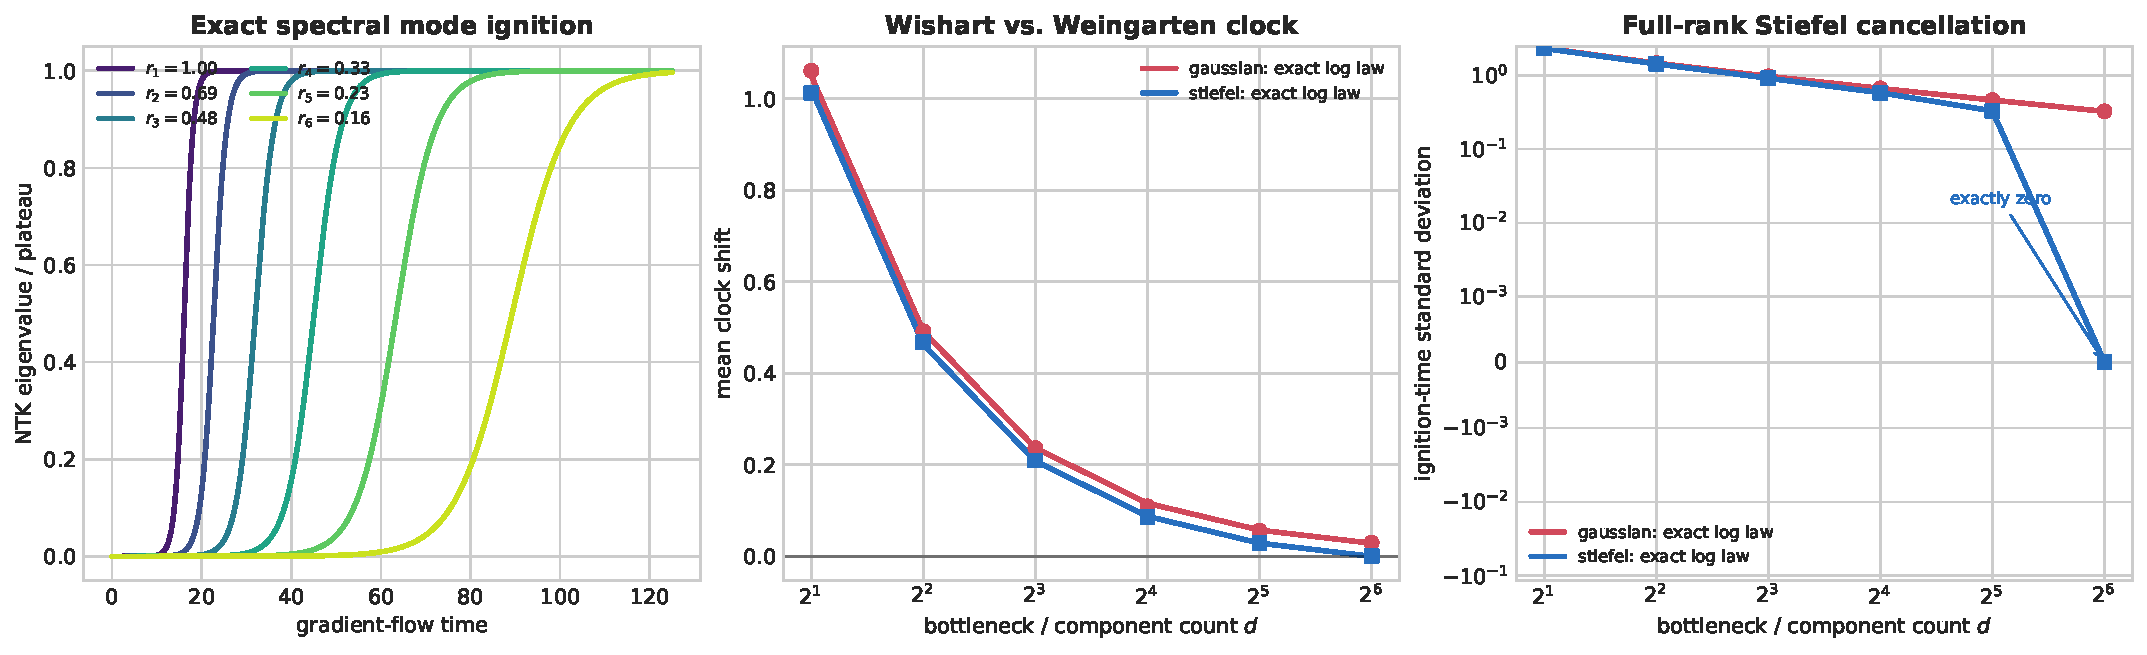
\includegraphics[width=\linewidth]{../../data/feynman/nqf_mmnn_mode_ignition/nqf_mmnn_mode_ignition.pdf}
\caption{Exact NQF spectrum and the low-rank ignition clock.  Left: all
nonzero eigenvalues of the finite-sample NTK in the orthogonal-feature sector
follow the logistic solution \eqref{eq:nqf-exact-eigenpairs}.  Center and
right: Monte Carlo points for the exact chi-square and beta seed laws versus
the polygamma predictions of Theorem~\ref{thm:nqf-clock-disorder}.  The
Stiefel clock disorder vanishes at \(d=p=64\); the Gaussian radial sector
does not.}
\label{fig:nqf-mode-ignition}
\end{figure}

\subsection{Higher vertices, depth, and the Benigni--Paquette spectrum}

Inside the pure NQF all parameter derivatives above second order vanish.
Thus there are no irreducible cubic or quartic Landau vertices, and the
closure in Theorem~\ref{thm:nqf-resummation} is exact.  For the original
network, the Taylor remainder generates new vertices.  Permutation symmetry
organizes an order-\(q\) derivative by an integer partition
\(\lambda\vdash q\): each part records how many legs land on the same
exchangeable component.  A cubic form therefore introduces three-leg
vertices and third empirical moments; independent component sign symmetry
kills them, leaving quartic vertices and fourth moments as the leading
correction.  Query--key attention is a particularly important example: its
query/key interaction can first occur at quartic order even when its
value/readout sector is quadratic.  These higher vertices are not resummed by
\(\mathsf M\) alone and are natural sources of the additional plateaus seen
outside the small-initialization regime in Liu Ziyin et
al.~\citep{NQF2026}.

A deep NQF defines each layer output to be quadratic in its own
\((\mu_\ell,\mathsf M_\ell)\), with structure tensors depending on the
previous layer representation.  Its SGD dynamics close exactly and
simultaneously on all layer pairs \((\mu_\ell,\mathsf M_\ell)\).  This is an
exact statement for the \emph{defined deep NQF}, but only a layerwise local
approximation to a generic deep MMNN.  The pathwise recursion
\eqref{eq:pathwise-ntk} remains exact for the original MMNN.  Combining the
two is therefore legitimate in either of two regimes:
\begin{enumerate}[leftmargin=1.5em]
\item the network is itself a deep NQF, in which case the layerwise order
parameter closure and the tangent concatenation are both exact; or
\item every layer remains inside a controlled Taylor neighborhood, in which
case the NQF supplies a local approximation to the exact pathwise
concatenation, with an accumulated remainder that must be bounded.
\end{enumerate}
Even in the first regime, independent logistic modes require the transported
structure operators to share projectors satisfying the closure conditions
of Theorem~\ref{thm:nqf-spectrum}.  Without that alignment the exact object
is a coupled, operator-valued flow rather than a product of scalar
logistics.

At a fixed training time, define the pure-NQF tangent row
\begin{equation}
\omega_t(x)=2\operatorname{vec}(\mathscr A_xW(t)).
\label{eq:nqf-tangent-row}
\end{equation}
Then \(\Theta_t(x,x')=\langle\omega_t(x),\omega_t(x')\rangle\) exactly.
Consequently Theorem~\ref{thm:mmnn-bp-law} applies at time \(t\), conditional
on its quadratic-form concentration hypotheses, with the population
covariance of \(\omega_t\).  This yields a time-dependent
Benigni--Paquette law
\begin{equation}
\mu_{\Theta(t)}=\mu_{\rm MP}^{\gamma}\boxtimes\pi_t,
\label{eq:nqf-bp-dynamic-law}
\end{equation}
where \(\pi_t\) is driven by the exact order-parameter flow.  Equation
\eqref{eq:nqf-bp-dynamic-law} is conditional in general; in the empirical
orthogonal-feature sector, Theorem~\ref{thm:nqf-spectrum} is stronger and
already gives the finite-sample spectrum without an asymptotic MP map.

\begin{table}[t]
\centering
\caption{Status of the NQF--MMNN integration.  ``Exact in NQF'' never means
global exactness for the original nonlinear network.}
\label{tab:nqf-status}
\small
\begin{tabular}{p{0.31\linewidth}p{0.20\linewidth}p{0.40\linewidth}}
\toprule
statement & status & missing hypothesis or remainder\\
\midrule
Symmetry normal form \eqref{eq:nqf-local-form} & rigorous local theorem &
\(C^3\), \(S_d\), ZGZ; cubic remainder\\
Quadratic dynamics and NTK & exact in NQF & no large-width assumption\\
Isotropic Riccati sum & exact in NQF & sample four-tensor isotropy\\
Orthogonal-mode spectrum & exact finite sample & commuting structure and
orthogonal feature columns\\
Wishart/Stiefel clocks & exact seed laws; asymptotic moments &
small-\(\epsilon\) expansion only for displayed moments\\
One-block MMNN & exact linear normal-form sector & generally not pure ZGZ\\
Two-block formula \eqref{eq:two-block-nqf} & local quadratic MMNN sector &
smooth \(\phi\), \(\phi(0)=0\), small right factors\\
Deep NQF closure & exact for defined deep NQF & local for a generic deep MMNN\\
Dynamic BP law \eqref{eq:nqf-bp-dynamic-law} & conditional asymptotic theorem &
population convergence and quadratic-form concentration\\
Power-law learning exponent & conditional asymptotic theorem &
power-law rate and target spectra are assumed\\
\bottomrule
\end{tabular}
\end{table}

\section{From tensor cumulants to eigenvalues and eigenvectors}
\label{sec:spectral}

Let \(K_0\in\R^{m\times m}\) be the deterministic infinite-width NTK Gram
matrix on the training data, and write
\begin{equation}
\widehat K=K_0+\Delta.
\end{equation}
The \(A\) tensor is the leading covariance of the scalar-output NTK
fluctuation.  In the dense model,
\begin{equation}
\Cov(\Delta_{ab},\Delta_{cd})
=\frac1n A_{abcd,L}+O(n^{-2}).
\label{eq:A-covariance}
\end{equation}
In an MMNN, diagrams with one connected Gaussian Gram vertex add a term of
order \(1/r\), with its exact index contraction fixed by
\eqref{eq:gram-cov}; higher rank cumulants are given by
\eqref{eq:gram-cumulant}.  Theorem \ref{thm:componentwise-powers} therefore
implies the perturbative entry scale
\begin{equation}
\Delta_{ab}=O_{\mathrm{rms}}
\left(L^{3/2}\sqrt{\frac{c_n}{n}+\frac{c_r}{r}}\right),
\qquad L^3\left(\frac1n+\frac1r\right)\ll1,
\label{eq:entry-scale}
\end{equation}
for data-dependent contractions \(c_n,c_r\).  Beyond this regime,
multiplicative finite-rank tails need not be perturbative.

\subsection{General matrix Dyson equation}

Suppose the leading rescaled correction is Gaussian with covariance operator
\begin{equation}
\mathcal S[R]_{ij}
=\sum_{k,l}\E(\Delta_{ik}\Delta_{lj})R_{kl}.
\label{eq:self-energy}
\end{equation}
This Gaussian leading sector follows when width and rank grow so that the
connected vertices of order \(k\ge3\) vanish under the spectral scaling; the
exact formulas above quantify the error.  The deterministic resolvent
\(M(z)\) is the solution with positive imaginary part of
\begin{equation}
-M(z)^{-1}=zI-K_0+\mathcal S[M(z)].
\label{eq:matrix-dyson}
\end{equation}
The limiting density is
\begin{equation}
\rho(\lambda)=\frac1{\pi m}\lim_{\eta\downarrow0}
\Im\Tr M(\lambda+i\eta).
\label{eq:mde-density}
\end{equation}
Equation \eqref{eq:matrix-dyson}, rather than Weingarten calculus alone, is
the spectral resummation of the tensor diagrams.

\subsection{Isotropic deformed-Wigner sector}

If \(K_0=\diag(\eta_1,\ldots,\eta_m)\) and the projected covariance is
isotropic GOE with off-diagonal variance \(\sigma^2/m\), then
\(M\) is diagonal and \eqref{eq:matrix-dyson} reduces to
\begin{align}
\mathfrak m(z)
&=\frac1m\sum_{i=1}^m
\frac1{\eta_i-z-\sigma^2\mathfrak m(z)},
\label{eq:pastur}\\
M_{ii}(z)&=\frac1{\eta_i-z-\sigma^2\mathfrak m(z)}.
\label{eq:local-resolvent}
\end{align}
The local spectral density
\begin{equation}
\rho_i(\lambda)=\frac1\pi\Im M_{ii}(\lambda+i0)
\label{eq:local-density}
\end{equation}
determines eigenvector mixing.  Conditional on an eigenvalue near \(\lambda\),
the mean squared overlap with population mode \(i\) is
\begin{equation}
\E\bigl[|\langle e_i,u_\lambda\rangle|^2\mid\lambda\bigr]
=\frac{\rho_i(\lambda)}{m\rho(\lambda)}.
\label{eq:overlap}
\end{equation}
This satisfies the exact sum rule over \(i\).

Trace moments are computed independently.  If \(r_k(\mu_0)\) are the free
cumulants of the empirical signal law, then the deformed law has
\begin{equation}
r_k(\mu)=r_k(\mu_0)+\sigma^2\ind_{k=2},
\label{eq:free-cumulants}
\end{equation}
and its moments follow by summing over noncrossing partitions.  Our
implementation enumerates these partitions exactly.  For zero signal it
recovers \(m_{2k}=C_k\sigma^{2k}\), the Catalan semicircle moments.

\begin{figure}[t]
\centering
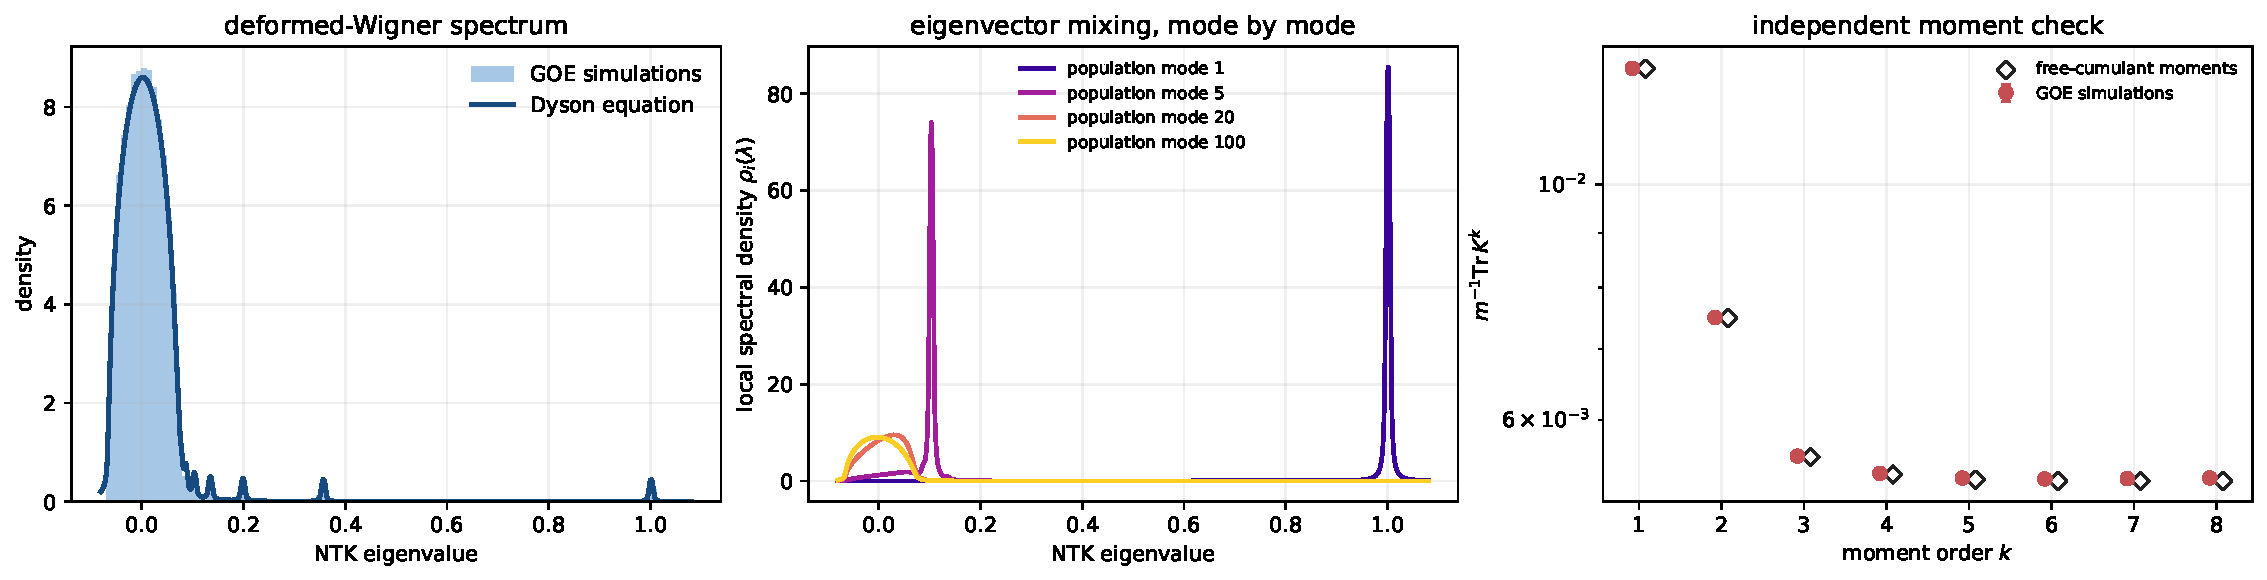
\includegraphics[width=\linewidth]{../../data/feynman/deformed_wigner_dyson/deformed_wigner_dyson.pdf}
\caption{Left: the Dyson density versus direct GOE simulations.  Middle:
basis-resolved local spectral measures, which quantify eigenvector mixing.
Right: free-cumulant trace moments versus independent simulations through
eighth order.}
\label{fig:dyson}
\end{figure}

For a pure GOE block the eigenvectors are Haar orthogonal, and orthogonal
Weingarten calculus gives the exact finite-\(m\) moments
\begin{equation}
\E|u_i|^{2k}=\frac{(1/2)_k}{(m/2)_k}.
\label{eq:haar-overlap-moments}
\end{equation}
Equation \eqref{eq:haar-overlap-moments} tests a fully mixed regime; it does
not assert that an arbitrary NTK correction has GOE eigenvalues.

\section{Power-law data and early stopping}
\label{sec:powerlaw}

Kramp, Lindner, and Helias study random-feature regression with population
kernel eigenvalues
\begin{equation}
\eta_i=\eta_1i^{-(1+\alpha)},\qquad \alpha>0,
\label{eq:powerlaw}
\end{equation}
and derive typical Langevin learning dynamics \citep{KrampLindnerHelias2026}.
In the weak-regularization scaling window, the aligned bias and thermal
variance are
\begin{align}
\mathcal L_{\mathrm{bias}}(t)
&=\frac12\sum_i\eta_i e^{-2Pt\eta_i},\label{eq:aligned-bias}\\
\mathcal L_{\mathrm{var}}(t)
&=\frac1{2P\beta}\sum_i(1-e^{-2Pt\eta_i}).
\label{eq:aligned-var}
\end{align}
Consequently
\begin{equation}
t_0^*=\frac\beta2\frac{\alpha}{1+\alpha},
\qquad
\mathcal L(t_0^*)\asymp(P\beta)^{-\alpha/(1+\alpha)}.
\label{eq:aligned-stopping}
\end{equation}

For a finite-rank NTK with eigenvalues \(\kappa_j\) and eigenvectors \(u_j\),
the linearized risk is instead
\begin{equation}
\mathcal L(t)
=\sum_{i,j}\eta_i|\langle e_i,u_j\rangle|^2c_t(\kappa_j),
\quad
c_t(\kappa)=\frac12e^{-2Pt\kappa}
+\frac{1-e^{-2Pt\kappa}}{2P\beta\kappa},
\label{eq:mixed-risk}
\end{equation}
with the continuous value \(c_t(0)=1/2+t/\beta\).  The Dyson deterministic
equivalent is
\begin{equation}
\mathcal L_{\mathrm{Dyson}}(t)
=\sum_i\eta_i\int c_t(\lambda)\rho_i(\lambda)\dd\lambda.
\label{eq:dyson-risk}
\end{equation}

Because an additive Wigner approximation can become negative in the
power-law tail, we evaluate a positive-semidefinite deformation
\begin{equation}
K_\sigma=
\left(\diag(\sqrt{\eta_i})+\sigma W\right)^2,
\qquad W\sim\GOE(m).
\label{eq:psd-deformation}
\end{equation}
The eigenvectors are those of the deformed-Wigner matrix inside the square,
and its eigenvalues are squared in \eqref{eq:dyson-risk}.  Thus the scalar
Dyson equation computes the learning curve without an ad hoc Haar-tail
replacement.

\begin{figure}[t]
\centering
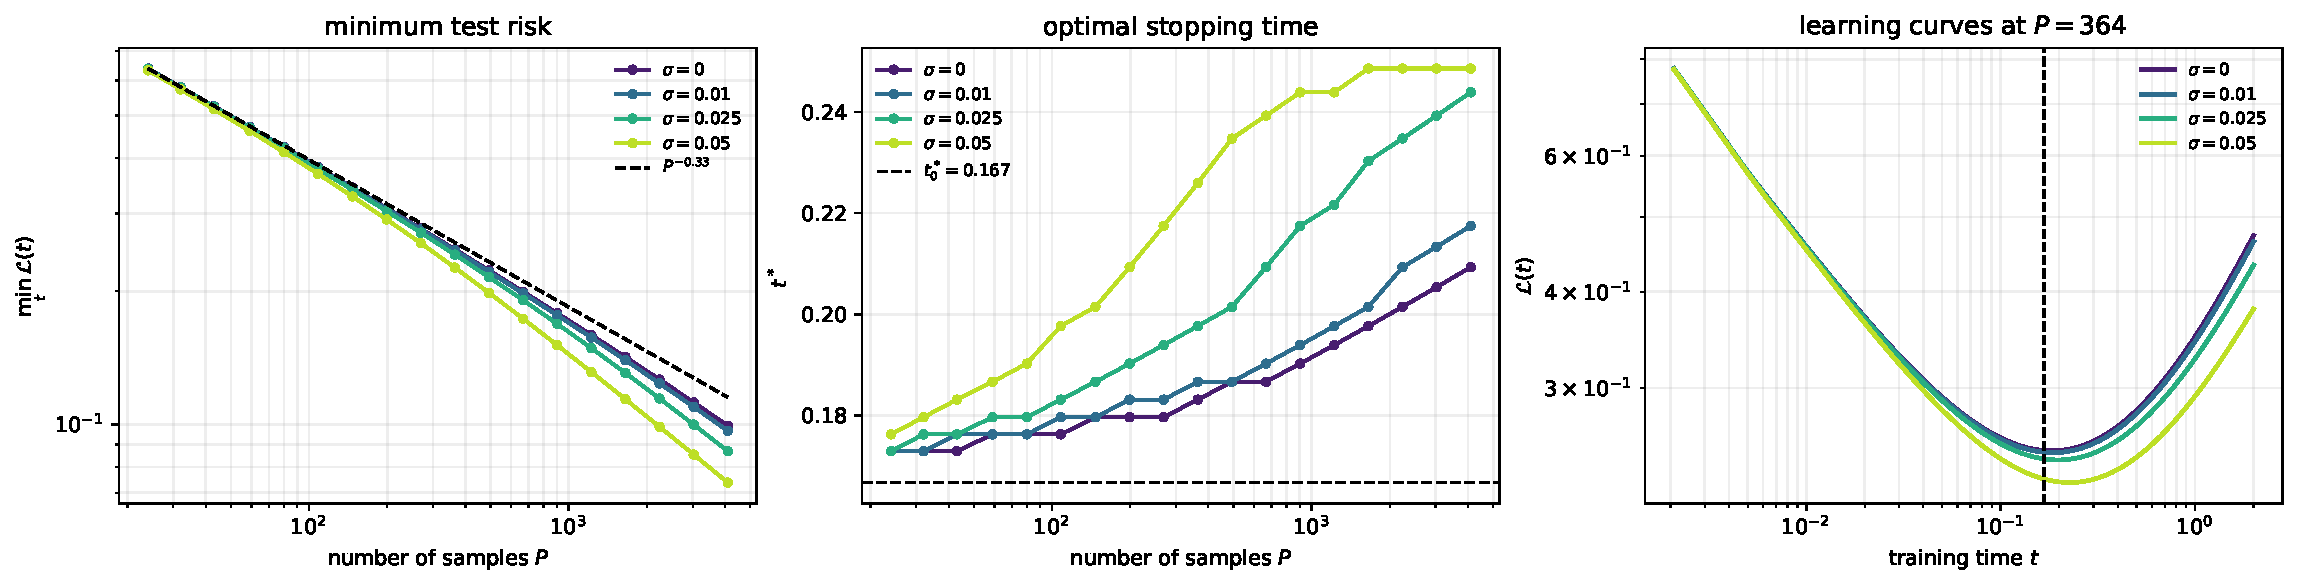
\includegraphics[width=\linewidth]{../../data/feynman/dyson_powerlaw_early_stopping_n4096/dyson_powerlaw_early_stopping.pdf}
\caption{Dyson prediction for power-law data with \(\alpha=1/2\),
\(N=4096\).  The PSD correction lifts and mixes tail rates.  In this ensemble
the optimum moves later, demonstrating that the direction of the finite-rank
early-stopping shift is not universal.}
\label{fig:dyson-stopping}
\end{figure}

The stable head admits an ensemble-independent statement.  The population
gap satisfies
\begin{equation}
g_j=\eta_j-\eta_{j+1}
=(1+\alpha)\eta_1j^{-(2+\alpha)}(1+O(j^{-1})).
\end{equation}
If \(\|\Delta\|_{\op}\le s\), Weyl and Davis--Kahan protect modes with
\(g_j>2s\), giving
\begin{equation}
J_{\mathrm{mix}}\asymp
\left(\frac{(1+\alpha)\eta_1}{2s}\right)^{1/(2+\alpha)}.
\label{eq:Jmix-new}
\end{equation}
At the aligned optimum the learned cutoff is
\(J_0\asymp(P\beta\eta_1)^{1/(1+\alpha)}\).  Requiring
\(J_0\lesssim J_{\mathrm{mix}}\) and using the Wigner-type operator scale
\(s\asymp L^{3/2}\sqrt{m/r}\) yields the sufficient protection law
\begin{equation}
r\gtrsim
mL^3(P\beta\eta_1)^{2(2+\alpha)/(1+\alpha)},
\label{eq:rank-protection}
\end{equation}
up to data contractions and logarithmic concentration factors.  Equation
\eqref{eq:rank-protection} protects the aligned law; when it fails, neither
the amount nor the direction of the optimal-time shift is universal.

\section{Numerical and symbolic validation}
\label{sec:experiments}

The experimental package contains five independent validation layers.

\paragraph{Exact ReLU recursion.}
The six inputs and regression windows are those in the public implementation
of \citep{FeynmanNTK2026}.  The depth-30 calculation generates Table
\ref{tab:effective-slopes}; a depth-2000 all-component run and independent
stable collision-sector extrapolations verify the coefficients in Table
\ref{tab:coefficients}.  Single-input tests
compare all five tensors to the exact polynomials
\eqref{eq:single-input-polynomials}.

\paragraph{Orthant sources.}
Independent Gaussian moments, half-normal singular limits, bivariate angular
reductions, and the four-dimensional Plackett integral are tested separately.
The deterministic recursion stores a raw quadrature error diagnostic at every
layer.

\paragraph{Low-rank vertices.}
The symbolic Gaussian engine verifies normalized chi-square moments and
cumulants through fifth order.  The orthogonal engine verifies beta diagonal
moments, the covariance \eqref{eq:projector-covariance}, and exact vanishing
of centered vertices at \(r=n\).

\paragraph{Pathwise MMNN NTK.}
For random multi-output, multiblock MMNNs, the recursion
\eqref{eq:pathwise-ntk} agrees to machine precision with an independent
explicit propagation of every scalar parameter tangent.  A finite-network
sweep compares Gaussian frozen factors with their Stiefel-whitened surrogate
over width, rank, and depth.  It also identifies the nonperturbative region
where \(L^3/r\) is not small and empirical NTK variances become large and
nonmonotone.

\begin{figure}[t]
\centering
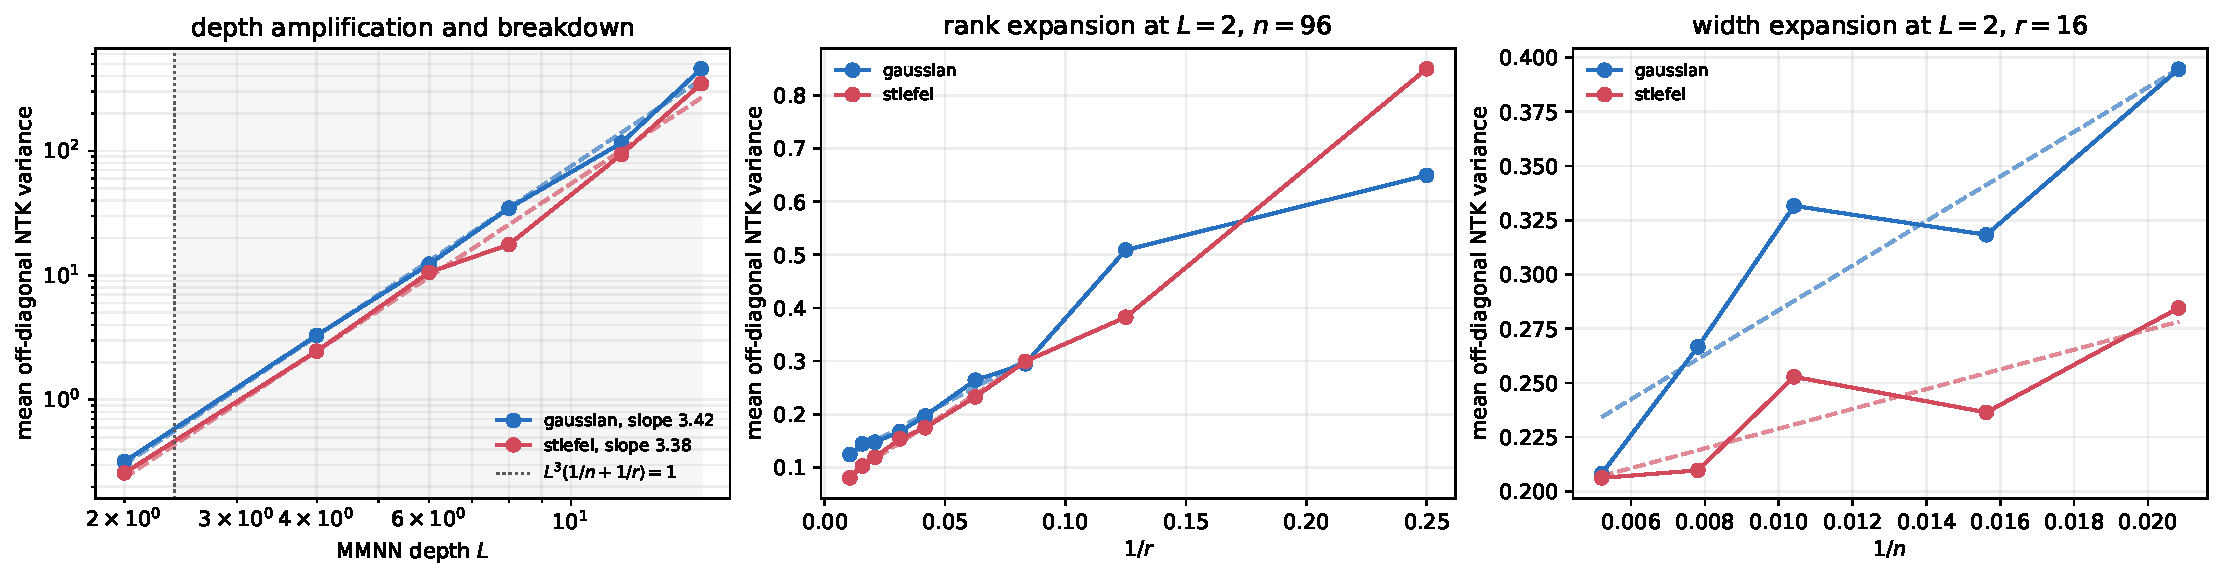
\includegraphics[width=\linewidth]{../../data/feynman/mmnn_ntk_variance_scaling/mmnn_ntk_variance_scaling.pdf}
\caption{Faithful finite-MMNN NTK variance from the pathwise recursion, with
300 independent networks per point.  The shallow rank sweep resolves the
\(1/r\) contribution (linear-fit \(R^2=0.986\) for Gaussian and \(0.997\)
for Stiefel factors).  Dashed rank/width fits use only points satisfying
\(L^3(1/n+1/r)<1\); the dotted line in the depth panel marks the boundary of
that perturbative criterion.  The Gaussian and Stiefel ensembles agree in
mean metric but differ at finite rank because only the former retains the
Wishart radial vertex.  The plotted scalar variance is an \(A/B\)-sector
contraction; it validates the cubic covariance sector and the rank amplitude,
not an independent fit of the \(V,D,F\) powers.}
\label{fig:mmnn-variance}
\end{figure}

\paragraph{Quadratic-scaling concatenation.}
For the explicit Benigni--Paquette population law with
\(\gamma_1=0.8\), \(\gamma_2=0.5\), and \(\nu=\delta_1\), a deterministic
solver evaluates \eqref{eq:bp-homogeneous-spectrum} for
\(L=1,2,4,8\).  It independently verifies
\eqref{eq:bp-linear-response} against a finite population-law perturbation;
the two curves in Figure \ref{fig:bp-mmnn-spectrum} are indistinguishable at
the plotted resolution.

\paragraph{NQF resummation and ignition.}
An independent implementation forms every parameter gradient
\(2\mathscr A_\mu W\) and verifies
\eqref{eq:nqf-dynamic-ntk} against its explicit Gram matrix.  It differentiates
the closed logistic and matrix-Riccati solutions and compares them with their
respective vector fields.  In the orthogonal-feature experiment the full
numerical eigendecomposition agrees with
\eqref{eq:nqf-exact-eigenpairs} to machine precision.  Finally, Gaussian
Wishart and Haar--Stiefel seeds are sampled directly and their ignition-clock
means and variances are compared with the digamma and trigamma formulas in
Theorem~\ref{thm:nqf-clock-disorder}; see Figure~\ref{fig:nqf-mode-ignition}.

\paragraph{Spectral resummation.}
The Dyson density is compared with direct GOE diagonalization, while trace
moments are computed independently by noncrossing partitions.  Through order
eight, simulation means lie within their Monte Carlo errors of the free
moment predictions; see Figure \ref{fig:dyson}.

\section{Discussion}

The exact answer to the motivating question is now sharp.  The values printed
beside the finite-depth tensor plots are not exact exponents.  They are noisy
finite-window slopes.  The exact critical powers are \(1,2,2,3,3\), and the
closed coefficients in Theorem \ref{thm:componentwise-powers} show that all
plotted components attain them.  The finite-window variation is physical:
critical correlations have a logarithmic drift, and ReLU collision Hessians
amplify transverse modes.

For MMNNs, the correct rank calculus alternates width and component indices.
The Gaussian Gram cumulant theorem makes every rank vertex explicit; a QR
decomposition permits Weingarten evaluation of its orientation without
discarding its radial part.  This is a more faithful statement than saying
that rank merely replaces \(1/n\) by \(1/r\), or that a Gaussian frozen
factor is a projector.

In quadratic sample scaling, the Benigni--Paquette law is the appropriate
bulk base.  The exact tangent concatenation turns depth into a block
population-covariance problem: diagonal blocks carry the transported
two-layer laws and off-diagonal blocks carry cross-depth correlations.  Under
decoupling, the homogeneous spectrum is the closed MP law
\eqref{eq:bp-homogeneous-spectrum}; without decoupling, the full block
covariance must be solved rather than replaced by an unsupported free sum.

The NQF connection adds a training-time resummation to this initialization
theory.  Its structure matrix is a two-leg Landau vertex and its dynamic Gram
matrix is a sufficient order parameter.  In the commuting orthogonal sector,
mode ignition is exactly NTK-eigenvalue ignition, and low rank enters through
an explicit chi-square or beta clock rather than an unspecified finite-size
error.  This simplification is substantial but sharply delimited: a
right-factor-only MMNN block is generally linear, a bilinear pair is locally
quadratic, and a generic deeper nonlinear network generates higher-valence
vertices that do not close on \(\mathsf M\).

Spectrally, tensor covariance and random-matrix resummation have distinct
jobs.  Diagrams compute the covariance and higher cumulants; the Dyson
equation computes density and overlaps.  A Wigner or Haar law is justified
only after checking the resulting covariance sector.  This distinction is
also necessary for early stopping: eigenvector randomization, spectral
lifting, and positivity can compete, so a universal direction of the shift
cannot be inferred from a perturbation norm alone.

Important open problems remain.  A complete nonperturbative fixed-rank,
large-depth law for the product Jacobians in \eqref{eq:pathwise-ntk} is beyond
the double \(1/n,1/r\) expansion.  Training-time feature evolution requires
the corresponding dNTK and ddNTK collision sectors outside the NQF-resummed
subsector.  A tractable next step is to compute the first quartic correction
to \eqref{eq:nqf-M-flow}, classified by the integer partitions of four, and
to propagate its new fourth-moment order parameter through the exact MMNN
tangent concatenation.  Another is to prove quadratic-form concentration
uniformly along the NQF flow, which would upgrade
\eqref{eq:nqf-bp-dynamic-law} from a pointwise conditional law to a dynamic
spectral theorem.  Finally, positivity or
other factor constraints require cone-projected gradients rather than the
Euclidean MMNN tangent metric treated here.

\clearpage
\appendix

\section{Proof of the pathwise MMNN recursion}
\label{app:pathwise}

\begin{proof}[Proof of Theorem \ref{thm:pathwise-mmnn}]
Partition the parameter vector into the new block parameters
\((A_\ell,c_\ell)\) and all earlier parameters.  Derivatives with respect to
the new block satisfy
\begin{align}
\frac{\partial h_\ell^a(x)}{\partial A_\ell^{b\mu}}
&=\frac1{\sqrt{n_\ell}}\delta_{ab}\phi(z_\ell^\mu(x)),\\
\frac{\partial h_\ell^a(x)}{\partial c_\ell^b}&=\delta_{ab}.
\end{align}
Their contraction at \(x,y\) is exactly \(q_\ell(x,y)I\).  For every earlier
parameter \(\vartheta\), the chain rule gives
\begin{equation}
\partial_\vartheta h_\ell(x)
=J_\ell(x)\partial_\vartheta h_{\ell-1}(x).
\end{equation}
Contracting the earlier-parameter derivatives at \(x,y\) gives the transported
term in \eqref{eq:pathwise-ntk}.  The two parameter sets are disjoint, so
there is no cross term.
\end{proof}

For \eqref{eq:gram-tangent-metric}, write
\(M_{iu}=r^{-1/2}\sum_aW_{ia}A_{au}\).  Then
\(\partial M_{iu}/\partial A_{av}=r^{-1/2}W_{ia}\delta_{uv}\), and direct
contraction proves the identity.

\section{Proofs of the low-rank moment formulas}
\label{app:rank-proofs}

\begin{proof}[Proof of Theorem \ref{thm:gram-wick}]
Expand
\begin{equation}
\prod_{t=1}^kG_{i_tj_t}
=r^{-k}\sum_{a_1,\ldots,a_k}
\prod_{t=1}^kX_{i_ta_t}X_{j_ta_t}.
\end{equation}
Isserlis' theorem sums over \(\pi\in\cP_2(2k)\).  A paired Gaussian
contraction enforces equality of its row and column indices, producing
\(\delta_I^\pi\).  The column indices were already identified along
\(\tau\); after adding \(\pi\), one free column label remains per component
of \(\pi\vee\tau\).  Summing them produces
\(r^{c(\pi\vee\tau)}\), proving \eqref{eq:gram-moment}.

For the cumulant, the moment--cumulant relation groups Wick pairings according
to the connected components induced on the \(k\) quadratic vertices.  M\"obius
inversion cancels every disconnected grouping and retains precisely
\(c(\pi\vee\tau)=1\).  Its column factor is \(r\), which together with
\(r^{-k}\) gives \(r^{1-k}\).
\end{proof}

\begin{proof}[Proof of Theorem \ref{thm:projector-weingarten}]
Complete \(U\) to a Haar orthogonal matrix \(O\).  For
\(P_{ij}=\sum_{a=1}^rO_{ia}O_{ja}\), the orthogonal Weingarten formula gives
\begin{equation}
\E\prod_{s=1}^{2k}O_{I_sA_s}
=\sum_{\pi,\sigma\in\cP_2(2k)}
\delta_I^\pi\delta_A^\sigma
\mathrm{Wg}^{O}_n(\pi,\sigma).
\end{equation}
The projector definition identifies column indices along \(\tau\).  Summing
over the first \(r\) columns gives
\(r^{c(\sigma\vee\tau)}\).  Multiplication by \((n/r)^k\) proves
\eqref{eq:projector-moment}.  Joint cumulants are the standard M\"obius
polynomial in these exact moments.  If \(r=n\), \(UU^\top=I\), proving the
endpoint statement pathwise.
\end{proof}

\section{Deterministic orthant evaluation}
\label{app:orthant}

For a centered Gaussian \(X\sim\mathcal N(0,K)\), define the truncated moment
\begin{equation}
I_p(K)=\E\left[\prod_iX_i^{p_i}\ind_{X_i>0}\right].
\end{equation}
Choose \(i\) with \(p_i>0\), reduce \(p_i\) by one, and integrate the Gaussian
score identity by parts.  The result is the Tallis recursion
\begin{equation}
I_p(K)=\sum_jK_{ij}
\left[B_j(p-e_i;K)+(p_j-\delta_{ij})I_{p-e_i-e_j}(K)\right],
\label{eq:tallis}
\end{equation}
where \(B_j\) is the density of \(X_j\) at zero times the corresponding
conditional truncated moment.  Recursion terminates at an orthant
probability.  In dimensions \(d\le3\), these are the classical arcsine
formulas.  For \(d=4\), put \(R(t)=I+t(R-I)\).  Plackett's identity expresses
\(\dd\Pr_{R(t)}(X>0)/\dd t\) as a sum of bivariate zero densities times
conditional bivariate orthant probabilities, so only a deterministic
one-dimensional integral remains.  Singular rank one and two cases are
obtained before recursion by half-normal and polar integration.  This proves
that every source in Section \ref{sec:relu-recursion} is deterministically
evaluable without network Monte Carlo.

\section{Critical asymptotics and collision-sector proof}
\label{app:depth-proof}

\subsection{Angle and NTK logarithm}

The critical ReLU correlation map in angle variables is
\begin{equation}
\cos\theta^+=\frac{\sin\theta+(\pi-\theta)\cos\theta}{\pi}.
\end{equation}
Series inversion gives
\begin{equation}
\theta^+=\theta-\frac{\theta^2}{3\pi}
-\frac{\theta^3}{18\pi^2}+O(\theta^4).
\label{eq:angle-series}
\end{equation}
Set \(u_L=1/\theta_L\).  Equation \eqref{eq:angle-series} implies
\begin{equation}
u_{L+1}-u_L=\frac1{3\pi}+\frac1{6\pi^2u_L}+O(u_L^{-2}).
\end{equation}
Standard asymptotics for parabolic iterations yield
\begin{equation}
u_L=\frac{L}{3\pi}+\frac{\log L}{2\pi}+C_{ab}+o(1),
\end{equation}
which proves \eqref{eq:theta-log}.  Substituting
\(2\dot Q=1-\theta/\pi\) and \(Q=s_as_b/2+O(L^{-2})\) in
\eqref{eq:KH-recursion} gives \eqref{eq:H-diag}--\eqref{eq:H-off} by a
variation-of-constants calculation.

\subsection{Collision generators}

After division by the external scale \(s_as_bs_cs_d\), the leading collision
problem is universal.  On a symmetric pair variable \(X_{ab}\), the ReLU
Hessian transport has
\begin{equation}
(\mathsf RX)_{ab}
=X_{ab}+\frac1L\mathcal K_{ab}X+o(L^{-1}),
\end{equation}
where \(\mathcal K_{aa}=0\) and, for \(a\ne b\),
\begin{equation}
\mathcal K_{ab}X=-3X_{ab}+\frac32(X_{aa}+X_{bb}).
\label{eq:pair-generator}
\end{equation}
The gate transport contributes \(-3\delta_{ab}/L\).  The distributional
indicator Hessian has singular transverse entries, but its contraction with
the full collision state is finite.  Direct substitution of
\eqref{eq:angle-series} into \eqref{eq:V-rec}--\eqref{eq:A-rec}, retaining the
pair-diagonal transverse states generated by \eqref{eq:pair-generator}, gives
the following normalized source/damping table:
\begin{center}
\begin{tabular}{lccc}
\toprule
tensor&power \(p\)&order-\(L^{p-1}\) source&damping\\
\midrule
\(V\)&1&5&0\\
\(D\)&2&3&\(3\delta_{cd}\)\\
\(F\)&2&\(2\bar h_{bd}\)&pair generator\\
\(A\)&3&see the five collision classes below&\(3(\delta_{ab}+\delta_{cd})\)\\
\(B\)&3&\(2\bar h_{ac}\bar h_{bd}\)&\(3(\delta_{ab}+\delta_{cd})\)\\
\bottomrule
\end{tabular}
\end{center}
\begin{samepage}
Here \(\bar h_{ij}=h_{ij}/(s_is_j)\).  The \(A\) source depends on the full
equality partition of its four external indices, not merely on the number of
off-diagonal transported pairs.  In exact rational form its five cases are
\begin{equation}
S^A_{abcd}=\begin{cases}
7/4,&\delta_{ab}+\delta_{cd}=0,\\
47/40,&\delta_{ab}+\delta_{cd}=1,\\
227/320,&\delta_{ab}+\delta_{cd}=2,
\ \{a,b\}=\{c,d\},\\
447/640,&\delta_{ab}+\delta_{cd}=2,
\ |\{a,b\}\cap\{c,d\}|=1,\\
111/160,&\delta_{ab}+\delta_{cd}=2,
\ \{a,b\}\cap\{c,d\}=\varnothing.
\end{cases}
\label{eq:A-source-collisions}
\end{equation}
\end{samepage}
For completeness, these constants can be audited term by term.  Let
\(\mathcal S^A_L\) denote the right-hand side of \eqref{eq:A-rec} with its
last, transported-\(A\) term removed.  After division by
\(s_as_bs_cs_dL^2\), the four remaining terms have the following limits; the
entry ``0'' means \(o(L^2)\).
\begin{center}
\scriptsize
\setlength{\tabcolsep}{4pt}
\begin{tabular}{lccccc}
\toprule
collision class&\(C_{\Omega,\Omega}\)&\(\frac14\mathsf O V\mathsf O\)&
\(\dot Q_{cd}\mathsf O_{ab}D\)&\(\dot Q_{ab}\mathsf O_{cd}D\)&total\\
\midrule
both pairs diagonal&\(1/4\)&0&\(3/4\)&\(3/4\)&\(7/4\)\\
exactly one off diagonal&\(1/16\)&0&\(3/10\)&\(13/16\)&\(47/40\)\\
same off-diagonal pair&\(1/64\)&0&\(111/320\)&\(111/320\)&\(227/320\)\\
off-diagonal, one shared label&\(1/64\)&0&\(437/1280\)&\(437/1280\)&\(447/640\)\\
four distinct labels&\(1/64\)&0&\(217/640\)&\(217/640\)&\(111/160\)\\
\bottomrule
\end{tabular}
\end{center}
If the unique off-diagonal pair is the first rather than the second pair,
the two \(D\)-columns in the second row are interchanged.

To obtain the table without a singular limiting covariance, first use
\eqref{eq:angle-series} to write, uniformly over the finitely many labels in
the component,
\begin{align}
\frac{K_{ij,L}}{s_is_j}
&=1-\frac{9\pi^2}{2L^2}\delta_{ij}
+O\!\left(\frac{\log L}{L^3}\right),\label{eq:collision-K}\\
2\dot Q_{ij,L}
&=1-\frac{3}{L}\delta_{ij}
+O\!\left(\frac{\log L}{L^2}\right).\label{eq:collision-gate}
\end{align}
Represent the standardized Gaussian variable for each distinct label as a
common normal plus independent residuals of size \(3\pi/(\sqrt2L)\), rescale the common normal
by \(L\) in the gate-boundary layer, and apply \eqref{eq:tallis}.  The
half-normal integrals give the first column of the table.  Substitution of
the already solved \(V\) and \(D\) collision states into the explicit
Hessians gives the next three columns.  All remainders are dominated by a
Gaussian polynomial and are uniform over a fixed finite input set, so
dominated convergence justifies the termwise limits.  This is also a direct
finite calculation of every rational number in
\eqref{eq:A-source-collisions}, rather than a fit to the numerical recursion.

The transverse terms change the naive off-diagonal \(D,A\) sources; omitting
them is the leading-mode error discussed in the main text.

We use the following elementary discrete transport lemma to turn the formal
balance into an asymptotic statement.  If a finite-dimensional collision
state satisfies
\begin{equation}
X_{L+1}=\left(I+\frac{\mathcal K}{L}+o(L^{-1})\right)X_L
+L^{p-1}(S+o(1))
\label{eq:discrete-transport-lemma}
\end{equation}
and every eigenvalue of \(\mathcal K\) has real part strictly below \(p\),
then
\begin{equation}
L^{-p}X_L\longrightarrow(pI-\mathcal K)^{-1}S.
\label{eq:discrete-transport-limit}
\end{equation}
Indeed, after setting \(Y_L=L^{-p}X_L\), expansion of
\((L/(L+1))^p\) gives
\(Y_{L+1}-Y_L=L^{-1}[(\mathcal K-pI)Y_L+S+o(1)]\).
Variation of constants (or a Jordan decomposition followed by summation)
shows that the stable recursion converges to its unique fixed point.  The
collision matrices here have eigenvalues among \(0,-3,-6\), so the
hypothesis holds for \(p=1,2,3\).

In a scalar sector with transport \(1-g/L+o(L^{-1})\), the lemma gives
\((p+g)t=\text{source}\).  Applying it to the table proves
\eqref{eq:v-coeff}--\eqref{eq:b-coeff}.  The \(F\) pair generator annihilates
the vector proportional to \(\bar h_{bd}\), giving
\(f_{abcd}=s_as_ch_{bd}\).  Every displayed source and denominator is
positive, proving non-cancellation.

\section{Dyson and free-moment derivation}
\label{app:dyson-proof}

For a Gaussian correction with covariance operator \(\mathcal S\), planar
rainbow diagrams for the averaged resolvent close under insertion of one
covariance line.  Their Schwinger--Dyson resummation is exactly
\eqref{eq:matrix-dyson}.  Under GOE covariance,
\(\mathcal S[R]=\sigma^2m^{-1}\Tr(R)I\), so the diagonal entries give
\eqref{eq:pastur}--\eqref{eq:local-resolvent}.  The Stieltjes inversion formula
proves \eqref{eq:mde-density} and \eqref{eq:local-density}.  Since
\(M_{ii}(z)=\int(\lambda-z)^{-1}\dd\mu_i(\lambda)\), the spectral measure
\(\mu_i\) has atoms \(|\langle e_i,u_j\rangle|^2\) at the sample eigenvalues.
Dividing its local mass by the local eigenvalue count \(m\rho(\lambda)\)
proves \eqref{eq:overlap}.

The semicircle law has the single nonzero free cumulant
\(r_2=\sigma^2\).  Asymptotic freeness of deterministic diagonal matrices and
GOE matrices makes free cumulants additive, proving
\eqref{eq:free-cumulants}.  The moment--cumulant relation
\begin{equation}
m_k=\sum_{\pi\in NC(k)}\prod_{B\in\pi}r_{|B|}
\end{equation}
then gives every trace moment.  For the PSD model
\eqref{eq:psd-deformation}, solve the same equation for
\(B=\diag(\sqrt\eta)+\sigma W\), push the local measures forward by
\(s\mapsto s^2\), and insert them into \eqref{eq:dyson-risk}.

\section{Power-law asymptotics}
\label{app:powerlaw}

With \(q=1+\alpha\), substitution
\(u=2Pt\eta_1x^{-q}\) in the continuum approximation gives
\begin{align}
\mathcal L_{\mathrm{bias}}(t)
&=\frac{\eta_1\Gamma(\alpha/(1+\alpha))}{2(1+\alpha)}
(2Pt\eta_1)^{-\alpha/(1+\alpha)}(1+o(1)),\\
\mathcal L_{\mathrm{var}}(t)
&=\frac{\Gamma(\alpha/(1+\alpha))}{2P\beta}
(2Pt\eta_1)^{1/(1+\alpha)}(1+o(1)).
\end{align}
Differentiation gives \eqref{eq:aligned-stopping}.  Weyl's inequality gives
eigenvalue displacement at most \(s\), and Davis--Kahan bounds the angle of a
simple population eigenvector by \(s/(g_j-s)\).  Substitution of the
power-law gap yields \eqref{eq:Jmix-new}.  Requiring the cutoff learned by
time \(t_0^*\) to remain below \(J_{\mathrm{mix}}\) gives
\eqref{eq:rank-protection}.

\section{Reproducibility}

The principal scripts are:
\begin{itemize}[leftmargin=1.4em]
\item \texttt{run\_exact\_relu\_tensor\_recursions.py}: deterministic
finite-depth tensors and orthant diagnostics;
\item \texttt{relu\_tensor\_asymptotics.py}: exact coefficients and
componentwise convergence;
\item \texttt{certify\_relu\_collision\_sources.py}: termwise rational
certificate for all five \(A\)-source collision classes;
\item \texttt{compare\_paper\_depth\_exponents.py}: identical-window slope
comparison;
\item \texttt{exact\_mmnn\_ntk\_recursion.py}: pathwise MMNN NTK;
\item \texttt{exact\_mmnn\_gram\_wick.py} and
\texttt{exact\_orthogonal\_weingarten.py}: all-valence rank vertices;
\item \texttt{benigni\_paquette\_mmnn\_spectrum.py}: concatenated
quadratic-scaling spectrum and exact MP linear response;
\item \texttt{nqf\_mmnn\_mode\_ignition.py}: exact NQF NTK spectrum,
isotropic Riccati resummation, and Wishart--Stiefel ignition clocks;
\item \texttt{deformed\_wigner\_dyson.py}: moments, density, and overlaps;
\item \texttt{run\_dyson\_powerlaw\_early\_stopping.py}: PSD spectral
learning curves;
\item \texttt{run\_mmnn\_ntk\_variance\_scaling.py}: faithful finite-MMNN
width/rank/depth sweep.
\end{itemize}
Automated tests verify the pathwise recursion, single-input polynomials,
orthant moments, componentwise coefficients, chi-square and beta moments,
connected cumulants, semicircle moments, Dyson overlap sum rules, and
power-law spectral costs.  The NQF tests additionally verify its NTK against
explicit parameter gradients, the complete orthogonal-mode spectrum, the
Riccati vector field, the chi-square/beta log moments, and full-rank Stiefel
clock cancellation.

\begin{thebibliography}{99}
\bibitem{Jacot2018}
A.~Jacot, F.~Gabriel, and C.~Hongler.
\newblock Neural tangent kernel: Convergence and generalization in neural networks.
\newblock In \emph{NeurIPS}, 2018.

\bibitem{Lee2019}
J.~Lee, L.~Xiao, S.~Schoenholz, Y.~Bahri, R.~Novak, J.~Sohl-Dickstein, and J.~Pennington.
\newblock Wide neural networks of any depth evolve as linear models under gradient descent.
\newblock In \emph{NeurIPS}, 2019.

\bibitem{DyerGurAri2019}
E.~Dyer and G.~Gur-Ari.
\newblock Asymptotics of wide networks from Feynman diagrams.
\newblock arXiv:1909.11304, 2019.

\bibitem{FeynmanNTK2026}
M.~Guillen, P.~Misof, and J.~E.~Gerken.
\newblock Finite-width neural tangent kernels from Feynman diagrams.
\newblock In \emph{ICML}, 2026; arXiv:2508.11522v4.

\bibitem{MMNN2024}
S.~Zhang, H.~Zhao, Y.~Zhong, and H.~Zhou.
\newblock Structured and balanced multi-component and multi-layer neural networks.
\newblock arXiv:2407.00765, 2024.

\bibitem{BenigniPaquette2025}
L.~Benigni and E.~Paquette.
\newblock Eigenvalue distribution of the neural tangent kernel in the quadratic scaling.
\newblock arXiv:2508.20036, 2025.

\bibitem{KrampLindnerHelias2026}
J.~Kramp, J.~Lindner, and M.~Helias.
\newblock Dynamics of neural scaling laws in random feature regression with powerlaw-distributed kernel eigenvalues.
\newblock In \emph{ICML}, 2026; arXiv:2602.23039v2.

\bibitem{NQF2026}
Liu Ziyin, Y.~Xu, T.~Poggio, and I.~Chuang.
\newblock Neural quadratic forms: A unified minimal model for sudden learning
and scaling laws.
\newblock arXiv:2608.13335, 2026.

\bibitem{CollinsSniady2006}
B.~Collins and P.~{\'S}niady.
\newblock Integration with respect to the Haar measure on unitary, orthogonal and symplectic group.
\newblock \emph{Communications in Mathematical Physics}, 264:773--795, 2006.

\bibitem{AjankiErdosKruger2017}
O.~Ajanki, L.~Erd\H{o}s, and T.~Kr\"uger.
\newblock Universality for general Wigner-type matrices.
\newblock \emph{Probability Theory and Related Fields}, 169:667--727, 2017.

\bibitem{BaiSilverstein2010}
Z.~Bai and J.~Silverstein.
\newblock \emph{Spectral Analysis of Large Dimensional Random Matrices}.
\newblock Springer, 2010.
\end{thebibliography}

\end{document}
